\chapter{Robust Feature Selection for Epigenetic Drift Characterisation}
\label{chap:feature_selection}


\section{Statistical Challenges of High-Dimensional DNA Methylation Data}
\label{sec:fs_hdlss}

The preprocessing framework developed in Chapter~\ref{sec:postproc_rationale} 
established a technically harmonised stabilised methylation space. 
However, preprocessing alone does not address the central statistical challenge 
of genome-wide DNA methylation data: extreme dimensionality relative to sample 
size. This challenge is particularly acute in the present study, where the 
objective is to characterise epigenetic differences along the 
Normal~$\to$~Adjacent~$\to$~Tumour axis in breast cancer — a setting in which 
biologically meaningful signal is expected to be subtle, spatially structured, 
and embedded in a feature space of several hundred thousand CpG loci.
High-throughput methylation arrays, such as the Illumina EPIC platform, 
interrogate approximately 850\,000 CpG sites per sample~\cite{Pidsley2016}, 
while the number of available subjects in any given cohort remains 
comparatively limited. This high-dimensional, low-sample-size (HDLSS) regime 
is well characterised in the statistical literature as a setting in which 
standard estimators become geometrically pathological: as dimensionality grows 
relative to $n$, pairwise distances concentrate, covariance estimation becomes 
unstable, and classifiers overfit to noise~\cite{Hall2005, Donoho2000}. In 
genomics specifically, the consequences are well documented — unconstrained 
feature spaces yield inflated classification accuracy that fails to replicate 
in independent cohorts~\cite{Ambroise2002, Smialowski2010}.
Feature selection is therefore not a cosmetic reduction step but a structural 
necessity for any learning procedure applied to molecular profiling data.

%-----------------------------------------------------------------------
\subsection{Structural Properties Motivating Feature Selection}
%-----------------------------------------------------------------------

Three properties of DNA methylation data collectively motivate explicit 
dimensionality control.

\paragraph{High Dimensionality and Overfitting Risk}
In HDLSS settings, discriminative models may achieve near-perfect separation 
on training data while capturing noise rather than biological signal. The 
phenomenon has been formally characterised by~\cite{Hall2005}, who showed 
that in very high dimensions, data from distinct classes become approximately 
equidistant unless genuine low-dimensional structure is present. Practically, 
this means that feature selection must precede, not follow, model fitting — 
and must itself be performed exclusively on training data to avoid 
optimistic bias~\cite{Ambroise2002}.

\paragraph{Spatial Correlation and Redundancy}
CpG loci exhibit strong local correlation driven by genomic proximity, 
chromatin organisation, and shared regulatory context. This spatial 
autocorrelation has been well characterised in large-scale mapping studies: 
contiguous CpGs within co-methylated blocks (``methylation domains'') 
can span hundreds to thousands of base pairs and behave as single 
epigenetic units~\cite{Hansen2011, Aryee2014}. Without explicit redundancy 
control, learning algorithms may over-represent densely correlated genomic 
regions while underweighting distributed epigenetic signals. This is 
especially relevant here, as differentially methylated regions (DMRs) 
along the Normal–Adjacent axis are expected to be spatially clustered 
rather than randomly distributed~\cite{Luo2018}.

\paragraph{Biological Sparsity}
Disease-associated methylation alterations are typically sparse and 
structured. In breast cancer, systematic analyses have demonstrated that 
tumour-associated hypermethylation preferentially targets specific regulatory 
programmes — including Polycomb-repressed developmental genes and 
oestrogen-regulated loci — while genome-wide methylation changes in 
histologically normal adjacent tissue are more subtle but nonetheless 
detectable~\cite{Teschendorff2016, Fleischer2017}. This sparsity 
motivates filtering strategies that prioritise stable, biologically 
coherent CpG subsets over exhaustive feature retention.

%-----------------------------------------------------------------------
\subsection{Methodological Challenges in Genomic Feature Selection}
%-----------------------------------------------------------------------
\label{subsec:fs_stability}
Feature selection in genomic data presents challenges that go beyond 
simple variable ranking.

\paragraph{Information Leakage}
The most consequential pitfall is information leakage: when feature 
selection is performed on the full dataset prior to cross-validation, 
the evaluation procedure has implicitly seen the test labels during 
variable ranking. \cite{Ambroise2002} demonstrated empirically that 
this leakage can inflate estimated accuracy by 10–40 percentage points 
in gene expression data; analogous inflation has been documented for 
methylation-based classifiers~\cite{Smialowski2010}. Strict containment 
of all selection steps within the training fold is therefore essential 
and is enforced throughout the present framework.

\paragraph{Significance Versus Stability}
A second challenge concerns the relationship between statistical 
significance and effect stability. In large feature spaces, extremely 
small $p$-values may arise for negligible or unstable effect sizes — a 
manifestation of the multiple testing problem that is not fully 
resolved by correction alone~\cite{Gelman2014}. Conversely, 
biologically relevant features may show moderate but reproducible 
signal across subsamples. Stability selection~\cite{Meinshausen2010} 
addresses this by quantifying the reproducibility of feature inclusion 
across repeated subsampling, providing selection frequency as a 
complementary criterion to statistical rank.

\paragraph{Predictive Optimisation Versus Interpretability}
A third challenge is the tension between predictive optimisation and 
interpretability. Aggressive feature selection driven solely by 
discriminative performance may yield compact but biologically opaque 
models, while overly conservative selection may retain sufficient 
redundancy to obscure the underlying regulatory architecture. In 
translational contexts, this tension has additional implications: 
in-silico classification accuracy does not automatically imply 
clinical utility~\cite{Poste2011}, and the biological coherence of 
the selected feature set is therefore a criterion in its own right.


%-----------------------------------------------------------------------
\subsection{Design Objectives of the Selection Framework}
%-----------------------------------------------------------------------
\label{sec:fs_stability}

In light of the statistical and biological considerations discussed above,
the feature selection strategy developed in this chapter is designed to
satisfy four interconnected objectives. First, strict leakage control
ensures that all selection procedures are confined to training data,
preventing inflation of evaluation metrics through inadvertent information
exposure. Second, stability enforcement guarantees that CpGs are retained
only if they demonstrate reproducible discriminative behaviour across
repeated stratified resampling, ensuring robustness to training-set
perturbations. Third, redundancy reduction through correlation-based
pruning limits the over-representation of co-methylated genomic blocks
and promotes independent signal components. Fourth, genomic diversification
imposes structural constraints to prevent excessive concentration of
selected features within specific chromosomes or regulatory contexts.
The hyperparameters governing each stage of the pipeline — including
variability thresholds, stability cutoffs, correlation bounds, and
diversification budgets — were fixed based on domain knowledge and
methodological precedent rather than systematic optimisation. A formal
sensitivity analysis lies outside the scope of the present work and is
identified as a direction for future investigation in
Chapter~\ref{chap:conclusion_future_work}.

The objective is therefore not merely dimensionality reduction, but the
identification of a stable, biologically coherent, and generalisable CpG
subset capable of characterising the Normal--Adjacent epigenetic transition
and supporting cross-dataset validation.

%-----------------------------------------------------------------------
\section{General Feature Selection Framework}
\label{sec:fs_framework}
%-----------------------------------------------------------------------

Building upon the statistical considerations outlined above, this section 
formally describes the feature selection workflow adopted in the present 
study. The procedure operates on the post-preprocessing methylation 
matrices defined in Chapter~\ref{chap:data_preprocessing} and is structured 
as a sequence of strictly train-only operations. These steps progressively 
reduce dimensionality while preserving statistical validity, stability, 
and biological coherence. From variability screening and scale 
transformation to stability-based ranking and redundancy control, 
each component addresses a specific structural property of DNA 
methylation data, culminating in a diversified CpG subset suitable 
for downstream cross-dataset evaluation.
%-----------------------------------------------------------------------
\subsection{Empirical Variability-Based Dimensionality Reduction}
\label{subsubsec:fs_initial_filter}
%-----------------------------------------------------------------------

The first stage of the feature selection framework consists of an 
unsupervised dimensionality reduction step aimed at removing CpGs 
that exhibit negligible variability within the tissue under study. 
This strategy is grounded in the empirically driven data reduction 
method proposed by \cite{Edgar2017}, who demonstrated that a 
substantial fraction of CpGs interrogated by the Illumina 450K array 
are effectively non-variable within a given tissue context, 
contributing to the multiple testing burden — by inflating the number of
hypotheses tested — without increasing the probability of detecting
true differential methylation signals.

\paragraph{Data restriction and structural cleaning}

Let$\mathcal{D} = \{(x_i, y_i)\}_{i=1}^{n}$,
where $x_i \in [0,1]^p$ represents the vector of $\beta$-values 
for $p$ CpG loci and $y_i \in \{0,1\}$ encodes the binary 
Normal--Adjacent label, with $y_i = 0$ denoting histologically 
normal tissue and $y_i = 1$ denoting tumour-adjacent tissue. 
Samples belonging to other tissue states (e.g.\ Tumour) are 
excluded from $\mathcal{D}$ prior to feature selection. 
This restriction ensures that the selected CpGs specifically 
characterise early epigenetic alterations occurring in 
histologically normal tissue adjacent to tumour, rather than 
late-stage tumour-specific methylation changes.

\paragraph{Train--test partition}

The dataset is partitioned into a training set 
$\mathcal{D}_{\mathrm{train}}$ and a held-out test set 
$\mathcal{D}_{\mathrm{test}}$ via stratified random sampling:
\begin{equation}
    \mathcal{D} = \mathcal{D}_{\mathrm{train}} \cup 
    \mathcal{D}_{\mathrm{test}}, 
    \quad 
    |\mathcal{D}_{\mathrm{train}}| = 0.80\,n, 
    \quad 
    |\mathcal{D}_{\mathrm{test}}| = 0.20\,n,
    \label{eq:split}
\end{equation}
with class proportions preserved in both sets. Crucially, 
all feature selection statistics — including the variability 
filter defined below — are estimated exclusively on 
$\mathcal{D}_{\mathrm{train}}$ and the resulting CpG subset 
is applied unchanged to $\mathcal{D}_{\mathrm{test}}$. This 
design prevents information leakage and ensures that 
dimensionality reduction is statistically independent of 
evaluation~\cite{Ambroise2002}.

\paragraph{Definition of the variability statistic}

For each CpG $j \in \{1,\dots,p\}$, variability is quantified 
using the robust inter-quantile range statistic proposed 
by \cite{Edgar2017}:
\begin{equation}
    r_{\beta,j}
    =
    Q_{0.90}\!\left(\beta_{j} \mid 
    \mathcal{D}_{\mathrm{train}}\right)
    -
    Q_{0.10}\!\left(\beta_{j} \mid 
    \mathcal{D}_{\mathrm{train}}\right),
    \label{eq:rbeta}
\end{equation}
where $Q_{0.90}$ and $Q_{0.10}$ denote the empirical 90th 
and 10th percentiles of the $\beta$-value distribution 
computed across all samples in $\mathcal{D}_{\mathrm{train}}$, 
pooling both tissue classes. Note that $r_{\beta,j}$ measures 
population-level dispersion unconditional on class membership: 
it quantifies whether a CpG is variable across individuals 
at all, not whether it discriminates between tissue types.
A CpG is retained if and only if:
$
    r_{\beta,j} \geq \tau, 
    \; \tau = 0.05,
$
yielding the retained index set
$    \mathcal{J}_{\mathrm{Edgar}} 
    = 
    \left\{ j \in \{1,\dots,p\} : r_{\beta,j} \geq \tau \right\}.$
The threshold $\tau = 0.05$ corresponds to the empirical 
criterion introduced in \cite{Edgar2017}: CpGs exhibiting 
a population-level methylation range below 5\% were 
operationally defined as non-variable and excluded. 
In the original study, this filter removed approximately 
20--30\% of probes on the 450K array across diverse tissue 
types~\cite{Edgar2017}.

\paragraph{Interpretation and scope}

Because $r_{\beta,j}$ is computed without reference to class 
labels, this filtering step is strictly unsupervised: it 
cannot introduce label-dependent bias and is therefore safe 
to apply upstream of the stratified cross-validation 
framework described in Section~\ref{subsec:fs_stability}. 
Its function is orthogonal to subsequent supervised ranking 
steps — it defines the candidate space over which 
discriminative selection will operate, not the final 
feature set.
CpGs excluded by this criterion ($r_{\beta,j} < 0.05$) 
typically correspond to loci consistently hypo- or 
hypermethylated across individuals, frequently enriched 
in CpG islands and constitutively silenced promoter 
regions~\cite{Edgar2017, Bock2012}. Retaining such loci 
inflates the effective dimensionality of the feature space 
without contributing discriminative variance, exacerbating 
the HDLSS geometry. Low-variance independent filtering is a standard strategy in high-dimensional genomic analyses to reduce noise and improve statistical efficiency without compromising type I error control~\cite{Bourgon2010}.
From a statistical perspective, $|\mathcal{J}_{\mathrm{Edgar}}|$ 
defines the reduced multiple testing space on which all 
downstream differential methylation analyses and stability 
selection procedures are conducted. The CpG subset 
$\mathcal{J}_{\mathrm{Edgar}}$, estimated on 
$\mathcal{D}_{\mathrm{train}}$, is applied identically to 
$\mathcal{D}_{\mathrm{test}}$ prior to any evaluation 
(Equation~\ref{eq:split}), preserving strict 
train--test separation throughout.

%-----------------------------------------------------------------------
\subsection{Re-alignment to $M$-values and Residual Variance Regularisation}
\label{subsec:fs_m_realign}
%-----------------------------------------------------------------------

The empirical variability screening of Section~\ref{subsubsec:fs_initial_filter}
is carried out in $\beta$-space, preserving continuity with the original
inter-quantile dispersion criterion of \cite{Edgar2017}. This is consistent with
the dual-representation strategy of Section~\ref{subsec:step3}: $\beta$-values
are retained for biological interpretability, while $M$-values are adopted for
statistical modelling because their logit transformation substantially stabilises
the mean--variance relationship~\cite{Du2010}.
Once $\mathcal{J}_{\mathrm{Edgar}}$ has been determined exclusively on
$\mathcal{D}_{\mathrm{train}}$, the analysis transitions to the $M$-value
representation defined in Equation~\eqref{eq:mvalue}. The transformation is
applied deterministically to the post-Edgar $\beta$ matrices of both training
and test sets: no model parameters are estimated at this stage. For each retained
CpG $j \in \mathcal{J}_{\mathrm{Edgar}}$,
using the same numerical stabilisation constant introduced during preprocessing.
The CpG subset selected in $\beta$-space is transferred unchanged to $M$-space,
preserving strict train--test separation throughout.

\paragraph{Residual low-variance trimming (train-only)}

Although the Edgar filter removes CpGs with negligible population-level
dispersion in $\beta$-space, a residual fraction of near-constant loci may
survive after logit transformation. This occurs because the logit map is
nonlinear: loci with $\beta$-values concentrated near the boundaries of $[0,1]$
can exhibit low inter-quantile range yet produce near-constant $M$-values once
mapped to the real line. Retaining such loci inflates the effective dimensionality
of the covariance structure without contributing discriminative signal, which
is particularly detrimental in HDLSS settings.
To address this, the pipeline systematically discards the lowest
$\alpha$-quantile of CpGs ranked by their empirical standard deviation in
$M$-space on $\mathcal{D}_{\mathrm{train}}$. Letting $s_j$ denote this
standard deviation, the retained index set is
\begin{equation}
    \mathcal{J}_{\mathrm{var}}
    =
    \left\{
        j \in \mathcal{J}_{\mathrm{Edgar}} :
        s_j \geq Q_{\alpha}(s)
    \right\},
    \qquad
    \alpha = 0.02,
\end{equation}
corresponding to the removal of the bottom 2\% of CpGs by dispersion.
The step is unsupervised — class labels play no role — and introduces no
information leakage. The quantile threshold is estimated solely on
$\mathcal{D}_{\mathrm{train}}$; the resulting binary mask is then applied
unchanged to $\mathcal{D}_{\mathrm{test}}$, maintaining complete statistical
independence of the evaluation set.
The resulting set $\mathcal{J}_{\mathrm{var}}$ constitutes the final candidate
feature space entering the supervised discriminative ranking stage described
in Section~\ref{subsec:fs_stability}.

%-----------------------------------------------------------------------
\subsection{Biologically Weighted Stability Selection and Region-Level Consolidation}
\label{subsec:fs_stability_ranking}
%-----------------------------------------------------------------------

After structural dimensionality control 
(Sections~\ref{subsubsec:fs_initial_filter} 
and~\ref{subsec:fs_m_realign}), the feature space remains 
in the order of several hundred thousand CpGs. In HDLSS 
regimes, univariate ranking alone is insufficient: small 
perturbations in training composition can induce large 
instability in feature ordering, particularly when 
signal-to-noise ratios are 
moderate~\cite{Hall2005, Donoho2000}. To address this, we 
adopt a resampling framework that integrates statistical 
evidence, directional consistency, and biologically informed 
weighting across four sequential components.

\paragraph{Repeated Stratified Stability Framework}

Let $X \in \mathbb{R}^{n_{\mathrm{train}} \times p}$ denote 
the post-filtered $M$-value matrix and 
$y \in \{0,1\}^{n_{\mathrm{train}}}$ the binary 
Normal--Adjacent label. A Repeated Stratified $K$-Fold (RSKF) procedure is employed with $K=5$ folds and $R=10$ repetitions, yielding $S = 50$ train/validation splits. 
Repeated stratified resampling reduces the variance of 
estimated feature importance and mitigates selection 
instability arising from dependence on a single 
partition~\cite{Ambroise2002, Smialowski2010}.
For each split $s = 1,\dots,S$ and each CpG $j$, three quantities are computed exclusively on the training fold.
\begin{enumerate}
\item The signed mean difference
\(
\Delta M_{j}^{(s)} = \bar{M}_{1,j}^{(s)} - \bar{M}_{0,j}^{(s)}
\)
is computed for all CpGs as an effect-size measure.

\item To reduce computational burden in the HDLSS regime,
Mann--Whitney $U$ $p$-values are evaluated only for the top
$50{,}000$ CpGs ranked by $|\Delta M_{j}^{(s)}|$ within the
training fold; CpGs outside this subset are assigned
$p_{j}^{(s)} = 1$.
This two-stage procedure introduces a structural dependency
between prescreening and rank aggregation, since excluded CpGs
receive a conservative rank by construction rather than by
statistical evidence. The approximation is justified by the
width of the prefilter: retaining $50{,}000$ candidates
corresponds to approximately $6\%$ of the full feature space,
substantially exceeding the final selection target of $5{,}000$
CpGs and limiting the probability of excluding genuinely
discriminative loci.
The Mann--Whitney test is adopted as a rank-based nonparametric
procedure to avoid distributional assumptions and ensure
robustness to residual deviations from normality in
$M$-space~\cite{MannWhitney1947}.
\item The same signed difference is computed independently on the validation fold to assess directional reproducibility across the partition.
\end{enumerate}

\noindent Two rank statistics are then derived per split,
\(
r_{p,j}^{(s)} \; \text{(ascending rank of } p_{j}^{(s)}),\)
\(r_{|\Delta M|,j}^{(s)} \\ 
\text{(descending rank of } |\Delta M_{j}^{(s)}|),
\)
and averaged across splits:
\begin{equation}
\overline{r}_{p,j}
=
\frac{1}{S}\sum_{s=1}^{S} r_{p,j}^{(s)},
\qquad
\overline{r}_{\Delta M,j}
=
\frac{1}{S}\sum_{s=1}^{S} r_{|\Delta M|,j}^{(s)}.
\end{equation}
The combined statistical score is the equal-weight convex 
combination:
\begin{equation}
\mathrm{score}_{\mathrm{stat},j}
=
0.5\,\overline{r}_{p,j}
+
0.5\,\overline{r}_{\Delta M,j}.
\end{equation}
This rank aggregation follows a Borda-count-like scheme~\cite{Fagin2003}, in which equal-weight combination of complementary ranking criteria has been shown to reduce selection variance relative to either criterion alone~\cite{Dwork2001}.
The resulting statistical score is subsequently min--max normalised 
to the unit interval:
\[
\mathrm{score}_{\mathrm{stat},j}^{\mathrm{norm}}
=
\frac{
\mathrm{score}_{\mathrm{stat},j}
-
\min(\mathrm{score}_{\mathrm{stat}})
}{
\max(\mathrm{score}_{\mathrm{stat}})
-
\min(\mathrm{score}_{\mathrm{stat}})
}.
\]
Relying solely on $p$-values risks prioritising negligible 
but stable effects under large sample sizes, whereas 
magnitude-only ranking may overweight noisy large 
deviations. Combining both criteria mitigates this trade-off and is consistent with resampling-based stability principles in high-dimensional feature selection~\cite{Meinshausen2010}.

\paragraph{Directional Stability Constraint}

A CpG whose estimated effect direction reverses across 
resampling splits is unlikely to reflect a genuine, 
reproducible biological signal. We therefore impose a 
directional reproducibility criterion. For each CpG $j$, 
let $\mathrm{sign}_{\mathrm{train}}^{(s)}$ and 
$\mathrm{sign}_{\mathrm{val}}^{(s)}$ denote the signs of 
$\Delta M_j^{(s)}$ on the training and validation folds 
of split $s$, respectively. The directional stability 
score is:

\begin{equation}
\mathrm{stab}_{j}
=
\frac{
\#\!\left\{
s :
\mathrm{sign}_{\mathrm{train}}^{(s)} =
\mathrm{sign}_{\mathrm{val}}^{(s)} \neq 0
\right\}
}{
\#\!\left\{
s :
\mathrm{sign}_{\mathrm{train}}^{(s)} \neq 0
\ \text{and}\
\mathrm{sign}_{\mathrm{val}}^{(s)} \neq 0
\right\}
}.
\end{equation}
The directional stability score is computed as the proportion 
of resampling splits in which both training and validation 
folds exhibit non-zero effect direction and agree in sign. 
CpGs for which the denominator equals zero — i.e.\ all splits 
yield $\Delta M_j^{(s)} = 0$ on at least one fold — are 
assigned $\mathrm{stab}_j = 0$ by convention, rendering them 
ineligible for selection under the stability constraint.
Only CpGs with $\mathrm{stab}_{j} \geq 0.75$ are retained, requiring directional agreement in at least 75\% of the splits for which a non-zero effect direction is observed in both folds. 
The threshold of 0.75 is chosen in analogy with the selection frequency cutoff recommended by~\cite{Meinshausen2010}, where a 75\% 
inclusion rate across subsampling splits is identified as a conservative criterion for stable feature identification. The same numerical threshold is here applied to directional consistency rather than selection frequency, extending the stability principle from feature inclusion to effect reproducibility — a particularly relevant criterion when the target signal is moderate in magnitude, as expected for early epigenetic drift in histologically normal adjacent tissue.

\paragraph{Adaptive Effect-Size Filtering}

A global effect estimate is computed on the full training 
set,
\(
\Delta M_{j}^{\mathrm{full}}
=
\bar{M}_{1,j} - \bar{M}_{0,j},
\)
and a CpG is retained only if 
$|\Delta M_{j}^{\mathrm{full}}| \geq Q_{0.60}(|\Delta M^{\mathrm{full}}|)$. 
Rather than applying a fixed $\Delta M$ cutoff — which 
would be sensitive to inter-cohort differences in 
dispersion — this adaptive percentile-based criterion 
maintains scale invariance across datasets. A fallback to 
the 50th percentile is applied when the resulting 
candidate pool would otherwise be insufficient for 
downstream selection. Together with the directional 
stability constraint, this filter ensures that only CpGs 
with both reproducible direction and non-negligible 
magnitude reach the biological weighting stage.
The fallback to the 50th percentile is triggered whenever the resulting candidate pool contains fewer than 15,000 CpGs, ensuring sufficient capacity for the downstream consolidation stage.


\paragraph{Integration of Biological Priors}

Purely statistical ranking may underweight loci in 
regulatory regions known to mediate transcriptional 
control. Promoter-associated CpGs and CpG islands are 
well-established sites of regulatory methylation changes 
in cancer and early field 
effects~\cite{Hansen2011, Fleischer2017}. Each CpG is assigned a discrete biological prior weight 
$w_j \in \{1.00, 0.70, 0.50, 0.20\}$ according to its island 
and promoter annotation:
\begin{equation}
w_j =
\begin{cases}
1.00 & \text{Island + TSS} \\
0.70 & \text{Island only} \\
0.50 & \text{Promoter (TSS) only} \\
0.20 & \text{Other loci}
\end{cases}
\end{equation}
The discrete weights are subsequently min--max normalised 
to the unit interval, yielding $w_j^{\mathrm{norm}} \in [0,1]$. 
In order to prioritise biologically annotated loci while 
preserving a lower-is-better scoring convention, the 
biological contribution is defined as 
$1 - w_j^{\mathrm{norm}}$.
After min--max normalisation of the statistical score 
$\mathrm{score}_{\mathrm{stat},j}$, the final integrated score is
\begin{equation}
\mathrm{score}_{j}
=
(1 - \lambda)\,\mathrm{score}_{\mathrm{stat},j}^{\mathrm{norm}}
+
\lambda\,(1 - w_j^{\mathrm{norm}}),
\qquad
\lambda = 0.20.
\end{equation}
Min--max normalisation is applied independently to each 
component prior to combination, ensuring commensurability 
of scale. The procedure is sensitive to extreme values; 
however, given the large number of CpGs 
($|\mathcal{J}_{\mathrm{var}}| \gg 10^4$), the influence 
of individual outliers on the normalised distribution is 
expected to be negligible.
The coefficient $\lambda = 0.20$ reflects a deliberate design 
choice rather than an empirically optimised parameter: 
statistical evidence contributes 80\% of the integrated score, 
while the remaining 20\% provides modest upweighting for loci 
with established regulatory function in promoter methylation 
and transcriptional silencing~\cite{Jones2012}. The top 15,000 CpGs 
satisfying both the stability and adaptive effect-size 
constraints define the candidate feature pool passed to the 
next stage.

\paragraph{Region-Level Anchoring on CpG Islands}

CpGs are not independent genomic entities: spatially 
proximal loci within co-methylated blocks co-vary as 
coordinated regulatory 
units~\cite{Hansen2011}. Selecting isolated top-ranked 
probes therefore risks capturing stochastic single-probe 
fluctuations rather than coherent epigenetic events, 
which is particularly problematic when the signal of 
interest — early field-effect drift — is expected to 
manifest as concerted changes across regulatory domains.
To enforce spatial coherence, candidate CpGs are grouped 
by annotated CpG island. For each island containing at 
least two candidate CpGs, a region-level score is defined 
as:
\begin{equation}
\mathrm{region\_score}
=
\mathrm{median}(\mathrm{score}_j)
\times
\mathrm{fraction}_{\mathrm{stable}},
\end{equation}
where $\mathrm{fraction}_{\mathrm{stable}}$ denotes the proportion 
of CpGs within the island satisfying both 
$\mathrm{stab}_j \geq 0.75$ and 
$|\Delta M_{j}^{\mathrm{full}}| \geq \tau$, 
with $\tau$ denoting the adaptive effect-size threshold 
selected in the previous step (60th percentile or 50th percentile fallback). 
The multiplicative formulation jointly penalises islands in which 
either the median discriminative score is weak or the proportion of 
internally stable CpGs is low: an island driven by isolated 
high-scoring probes surrounded by unstable loci receives a 
substantially discounted region score, ensuring that anchored 
islands exhibit both statistical quality and internal coherence. 
Only islands with $\mathrm{fraction}_{\mathrm{stable}} \geq 0.60$ and at 
least two candidate CpGs are retained. From each such 
island, the top $m = 2$--$3$ CpGs are selected into an 
anchored pool; the remaining candidates form a 
complementary non-anchored set. This hierarchical 
consolidation reduces susceptibility to single-probe 
artefacts and aligns feature selection with the biological 
expectation that early epigenetic drift occurs in clustered 
regulatory domains rather than as isolated stochastic 
events.

%-----------------------------------------------------------------------
\subsection{Correlation-Based Redundancy Pruning and Graph-Theoretic Clustering}
\label{subsec:fs_corr_pruning}
%-----------------------------------------------------------------------

Despite stability filtering and region-level anchoring, the 
candidate feature space retains strong local correlation. DNA 
methylation levels exhibit pronounced spatial autocorrelation 
driven by genomic proximity, shared chromatin context, and 
coordinated regulatory control~\cite{Hansen2011, Aryee2014}: 
in high-density arrays such as EPIC, neighbouring CpGs within 
islands and promoter regions frequently co-vary as near-redundant 
blocks. Retaining multiple highly correlated loci inflates the 
effective dimensionality of the design matrix without increasing 
independent information content, inducing multicollinearity, 
unstable coefficient estimates, and variance inflation in 
downstream classifiers~\cite{Donoho2000, Hall2005}. Explicit 
correlation-based redundancy pruning is therefore applied to 
the candidate pool before passing it to the diversification 
stage.

\paragraph{Correlation Structure on Training Data}

Let $Z \in \mathbb{R}^{n_{\mathrm{train}} \times q}$ denote 
the $M$-value matrix restricted to the $q$ candidate CpGs, 
with each column standardised using training-set mean $\mu_j$ 
and standard deviation $s_j$:
\[
Z_{ij}
=
\frac{M_{ij} - \mu_j}{s_j}.
\]
where $s_j$ is the sample standard deviation computed with Bessel correction 
(ddof $=1$) on the training set. A small numerical constant is added in practice 
to prevent division by zero in degenerate cases.
The empirical Pearson correlation matrix is then:

\begin{equation}
C
=
\frac{1}{n_{\mathrm{train}} - 1}
Z^{\top} Z.
\label{eq:corr_matrix}
\end{equation}
Because columns of $Z$ are standardised to zero mean and unit sample variance, 
Equation~\eqref{eq:corr_matrix} coincides with the empirical Pearson 
correlation matrix estimated exclusively on $\mathcal{D}_{\mathrm{train}}$.
All quantities are estimated exclusively on 
$\mathcal{D}_{\mathrm{train}}$ to preserve strict 
evaluation independence.

\paragraph{Graph Construction and Connected Components}

An undirected graph $G = (V, E)$ is constructed with one 
vertex per candidate CpG; an edge connects $j$ and $k$ 
whenever their absolute correlation exceeds the threshold:

\begin{equation}
(j,k) \in E
\;\Longleftrightarrow\;
|C_{jk}| \geq \tau_c,
\qquad
\tau_c = 0.85,
\label{eq:corr_graph}
\end{equation}
consistent with strong-correlation redundancy thresholds 
commonly adopted in high-dimensional omics 
analyses~\cite{Witten2010, Friedman2010}. By convention, each vertex is connected to itself in the adjacency matrix; 
this does not alter the connected component structure but simplifies 
implementation. Clusters are 
defined as the connected components of $G$: a cluster 
$\mathcal{C}$ is a maximal vertex subset in which every 
pair $(j,k)$ is joined by at least one path in $G$.
This graph-theoretic formulation is strictly preferable 
to pairwise sequential pruning because correlation 
propagates transitively: two CpGs with $|C_{jk}| < \tau_c$ 
may both be strongly correlated to a third, and would 
therefore represent the same co-methylated block without 
being linked directly. Connected components capture this 
transitive redundancy structure in a single, consistent pass.

\paragraph{Representative Selection per Cluster}

For each connected component $\mathcal{C}_m$, a single 
representative CpG is retained:

\begin{equation}
j^*
=
\arg\min_{j \in \mathcal{C}_m}
\,\mathrm{score}_j,
\label{eq:cluster_rep}
\end{equation}
where $\mathrm{score}_j$ is the integrated biologically 
weighted stability score of 
Section~\ref{subsec:fs_stability_ranking}, in which a 
lower value denotes stronger statistical and biological 
evidence. CpGs lacking a valid stability score are assigned an infinite value and are 
therefore ineligible for selection as cluster representatives. Selecting the minimum thus retains the most 
discriminative and stable CpG within each correlated 
block, discarding all redundant co-varying loci. While region-level anchoring leverages genomic annotation to enforce spatial 
coherence based on CpG island structure, the present clustering step operates 
purely on empirical covariance structure estimated from the training data.

\paragraph{Separate Clustering of Anchored and Non-Anchored Pools}

To preserve the island-level spatial structure established 
by region-level anchoring before applying global redundancy 
reduction, clustering is performed separately on the 
region-anchored pool $A$ (CpGs selected via island 
consolidation) and the non-anchored complementary pool 
$B$. Let $\mathcal{R}_A$ and $\mathcal{R}_B$ denote the 
representative sets obtained from each pool. Representatives 
from $A$ are prioritised in the final union, and the 
redundancy-pruned feature set is:
\(
\mathcal{R}
=
\mathcal{R}_A
\cup
\mathcal{R}_B.
\)

\paragraph{Statistical and Biological Rationale}

From a bias--variance standpoint, removing highly 
correlated predictors reduces estimator variance while 
preserving most of the predictive signal, since strongly 
correlated CpGs encode largely overlapping epigenetic 
information. In HDLSS settings this is particularly 
consequential: redundant features exacerbate the 
ill-conditioning of the design matrix, inflate effective 
model complexity, and destabilise decision 
boundaries~\cite{Donoho2000}. Removing redundant predictors reduces effective dimensionality 
and improves the numerical conditioning of the design matrix 
without materially reducing predictive information content.
The result is a structurally compact, non-redundant 
feature set that retains statistical strength, directional 
stability, biological coherence, and spatial structure — 
forming the input to the genomic diversification stage 
described in Section~\ref{subsec:fs_diversification}.

%-----------------------------------------------------------------------
\subsection{Genomic Diversification via Constrained Greedy Selection}
\label{subsec:fs_diversification}
%-----------------------------------------------------------------------

After correlation-based redundancy pruning
(Section~\ref{subsec:fs_corr_pruning}), the feature set
$\mathcal{R}$ remains enriched for highly ranked CpGs but
may still exhibit structural imbalance. Genome-wide methylation
arrays are inherently non-uniform — CpG density varies
substantially across chromosomes, islands, shores, shelves, and
open sea regions — so unconstrained greedy ranking tends to
over-concentrate features in CpG-dense promoter islands,
high-signal chromosomes, and local windows of coordinated drift.
Such concentration reduces effective genomic coverage and
increases the risk that downstream models capture locus-specific
rather than system-level epigenetic patterns, undermining
structural generalisability across cohorts. A diversification
step is therefore introduced as a constrained subset selection
problem.

\paragraph{Problem Formulation}

Let $\mathcal{R} = \{j_1, \dots, j_m\}$ denote the 
redundancy-pruned CpG pool ordered by increasing 
integrated score $\mathrm{score}_j$ 
(Section~\ref{subsec:fs_stability_ranking}).
CpGs lacking valid manifest annotation for chromosome and genomic position 
are excluded prior to diversification, as spatial constraints require 
coordinate information.
The goal is to select a subset
\(
\mathcal{S} \subset \mathcal{R},
\;
|\mathcal{S}| = K = 5000,
\)
that maximises overall discriminative quality under 
structural diversity constraints. In practice, the effective target is defined as 
$K_{\mathrm{eff}} = \min(K, |\mathcal{R}|)$ 
to accommodate cases in which fewer than $K$ mapped CpGs are available; 
all constraint budgets are computed with respect to $K_{\mathrm{eff}}$.
The target cardinality $K = 5000$ represents approximately 
$1.0\%$ of the probes interrogated by the Illumina 450K array 
and approximately $0.6\%$ of those interrogated by the EPIC array. 
It is selected to provide sufficient genomic coverage for 
cross-cohort evaluation while maintaining a feature-to-sample 
ratio compatible with stable supervised learning in the 
available cohorts. The choice is acknowledged as a design 
parameter rather than an optimised quantity; its sensitivity 
is identified as a direction for future investigation in 
Chapter~\ref{chap:conclusion_future_work}. %In practice, the effective target is defined as 
%$K_{\mathrm{eff}} = \min(K, |\mathcal{R}|)$ 
%to accommodate cases in which fewer than $K$ mapped CpGs are available. 
%All constraint budgets are computed with respect to $K_{\mathrm{eff}}$.
Formally:
\begin{equation}
\label{eq:div_problem}
\begin{aligned}
\min_{\mathcal{S} \subseteq \mathcal{R}} 
\quad & \sum_{j \in \mathcal{S}} \mathrm{score}_j 
\\
\text{s.t.} \quad 
& |\mathcal{S}| = K_{\mathrm{eff}}, 
\\
& |\{ j \in \mathcal{S} : c(j)=\chi \}| 
  \leq \lfloor \alpha_{\mathrm{chr}} K_{\mathrm{eff}} \rfloor 
  \quad \forall \chi,
\\
& |\{ j \in \mathcal{S} : \gamma(j)=g \}| 
  \leq \lfloor \alpha_{\mathrm{ctx}} K_{\mathrm{eff}} \rfloor 
  \quad \forall g,
\\
& |\{ j \in \mathcal{S} : w(j)=\omega \}| 
  \leq \beta 
  \quad \forall \omega.
\end{aligned}
\end{equation}
Each constraint targets a distinct axis of potential 
structural imbalance and is described in turn below.

\paragraph{Chromosomal Balance Constraint}

Let $c(j)$ denote the chromosome of CpG $j$. No 
chromosome may contribute more than a fixed fraction of 
the final set:

\begin{equation}
|\{ j \in \mathcal{S} : c(j) = \chi \}|
\leq
\alpha_{\mathrm{chr}} K,
\qquad
\alpha_{\mathrm{chr}} = 0.08.
\label{eq:chr_constraint}
\end{equation}
The budget per chromosome is computed as 
$\lfloor \alpha_{\mathrm{chr}} K_{\mathrm{eff}} \rfloor$, 
with a minimum of one CpG allowed per chromosome.
The 8\% cap prevents over-representation of chromosomes 
that harbour dense signal regions, a configuration known 
to affect classifier stability when disease-associated loci 
cluster in specific chromosomal domains~\cite{Witten2010}.

\paragraph{Genomic Context Constraint}
Let $\gamma(j)$ denote the CpG island context of locus 
$j$ (Island, Shore, Shelf, or OpenSea). The fraction of 
any single context class is bounded by:

\begin{equation}
|\{ j \in \mathcal{S} : \gamma(j) = g \}|
\leq
\alpha_{\mathrm{ctx}} K,
\qquad
\alpha_{\mathrm{ctx}} = 0.65.
\label{eq:context_constraint}
\end{equation}
The context budget is computed as 
$\lfloor \alpha_{\mathrm{ctx}} K_{\mathrm{eff}} \rfloor$, 
with at least one CpG permitted per context class.
Although promoter islands are biologically important, 
cancer-related methylation changes are not confined to 
islands and frequently involve shores and open sea 
regions~\cite{Hansen2011, Fleischer2017}. The soft cap 
ensures that non-island regulatory regions retain 
representation in the final panel.

\paragraph{Spatial Window Constraint}

To prevent local hyper-concentration, each chromosome is 
partitioned into non-overlapping windows of 
$W = 500\,\mathrm{kb}$, and the number of selected CpGs 
per window is hard-capped:
$|\{ j \in \mathcal{S} : w(j) = \omega \}|
\leq 15,$
where $w(j)$ is the window index of CpG $j$. Formally, windows are defined via integer binning 
$w(j) = \left\lfloor \mathrm{pos}(j) / W \right\rfloor$ 
within each chromosome. Since 
methylation domains frequently span tens to hundreds of 
kilobases~\cite{Hansen2011}, this constraint preserves 
regional representation while preventing dominance by a 
single hyper-variable block — a risk that correlation 
pruning alone cannot fully eliminate at the macro-scale.

\paragraph{Greedy Approximation with Progressive Relaxation}

The constrained optimisation problem~\eqref{eq:div_problem} 
is combinatorial and NP-hard in general, as it resembles 
cardinality-constrained subset selection with multiple 
linear constraints. Rather than solving a full 
mixed-integer program, we adopt a deterministic greedy 
strategy: CpGs are processed in order of increasing 
$\mathrm{score}_j$, ties are resolved deterministically by stable ordering, and each candidate is added to 
$\mathcal{S}$ if and only if all active constraints are 
simultaneously satisfied, until $|\mathcal{S}| = K$.
If the strict constraint regime fails to reach $K$, constraints are relaxed by staged deactivation (rather than by increasing thresholds), first removing the spatial window constraint, then the genomic context constraint, and finally the chromosome balance constraint.
At each stage, the specified constraint is fully deactivated while 
previously relaxed constraints remain inactive.
Spatial over-concentration is relaxed first because 
local genomic crowding is most detrimental to coverage; 
chromosomal imbalance is relaxed last as it has the 
weakest direct effect on independent information content. 
The constrained greedy strategy does not admit formal 
approximation guarantees in this setting, as the objective 
is linear rather than submodular and the constraint structure 
involves multiple simultaneous bounds. The approach is adopted 
as a computationally tractable heuristic; its empirical 
adequacy is assessed indirectly through the constraint 
activation frequency reported in 
Section~\ref{sec:fs_intra_dataset}.
The frequency with which progressive constraint relaxation is activated in practice is reported in Section~\ref{sec:fs_intra_dataset} for each dataset, allowing empirical assessment of whether the final selection approximates the fully constrained solution or degrades toward unconstrained score-based ranking.

% ============================================================
\section{Dataset-Specific Implementation}
\label{sec:fs_intra_dataset}
% ============================================================

This section documents the dataset-specific application of the feature selection framework described in Section~\ref{sec:fs_framework}. For each cohort, the outcome of empirical variability screening, $M$-value realignment and residual variance trimming, stability-based discriminative ranking with directional consistency constraints, redundancy reduction via correlation-graph clustering, and constrained genomic diversification is reported in detail. 

The results are presented separately for GSE69914 (Section~\ref{subsec:fs_intra_gse69914}), GSE225845 (Section~\ref{subsec:fs_intra_gse225845}), and GSE287331 (Section~\ref{subsec:fs_intra_gse287331}).

\subsection{Dataset GSE69914}
\label{subsec:fs_intra_gse69914}

The feature selection framework described in Section~\ref{sec:fs_framework} 
was applied to the preprocessed GSE69914 cohort, restricted to the 
Normal and Adjacent tissue classes, yielding a final panel of 
$K=5000$ CpGs after variability filtering, stability ranking, 
redundancy pruning, and diversification. The selected loci are 
available in the project repository at 
\href{https://github.com/elisabettaroviera/THESIS/blob/main/05%20-%20CpG%20list/Final%205000%20CpGs%20per%20Dataset/final_5000_gse69914.csv}
{\texttt{final\_5000\_gse69914.csv}}.

% ============================================================
\paragraph{Empirical Variability-Based Dimensionality Reduction}
% ============================================================

Variability was quantified via the inter-quantile range 
$r_{\beta,j} = P90(\beta) - P10(\beta)$ computed on the 
training set. Figure~\ref{fig:gse69914_variance_controls}(a) 
shows the empirical distribution of $r_{\beta}$ across CpGs. 
The distribution is strongly right-skewed, with a substantial 
mass concentrated below $r_{\beta}=0.05$. 
Applying the predefined threshold $\tau = 0.05$ removed 
100{,}103 low-variability loci, defining the reduced candidate 
space for downstream supervised ranking. Lower candidate 
thresholds (0.01, 0.02) are shown for reference but were not 
adopted, as they would retain a substantially larger fraction 
of near-constant probes. To assess whether this filtering step induced structural genomic bias,
the distribution of invariant loci across gene-feature categories
was examined via fold-change enrichment analysis.
As reported in Appendix~\ref{app:empirical_variability_extension},
invariant CpGs showed moderate enrichment in promoter-proximal
regions (TSS200, first exon, 5'UTR), whereas gene bodies and 3'UTR regions were relatively under-represented.
No extreme over-representation was observed, indicating that the
variability-based reduction primarily eliminates low-dispersion loci
without introducing pathological distortion of the genomic feature space.

% ============================================================
\begin{figure}[t]
\centering
\begin{subfigure}[t]{0.48\textwidth}
    \centering
    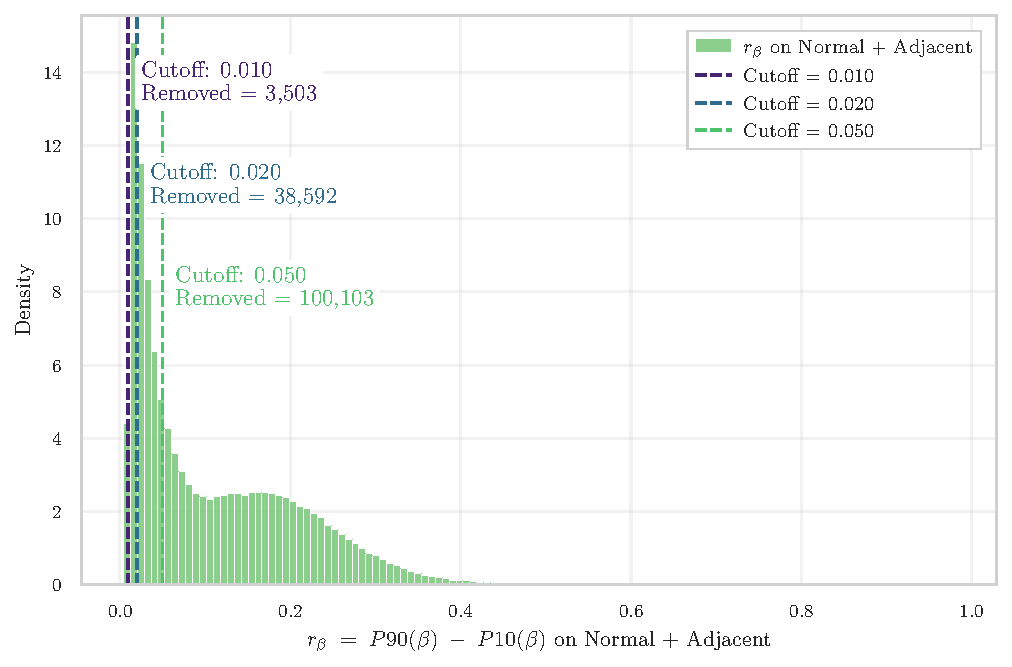
\includegraphics[width=\textwidth]{images/cap5/GSE69914_edgar_variability.pdf}
    \caption{$r_{\beta} = P90(\beta) - P10(\beta)$ 
    on the training set. Candidate thresholds 
    (0.01, 0.02, 0.05) are indicated.}
    \label{fig:gse69914_rbeta}
\end{subfigure}
\hfill
\begin{subfigure}[t]{0.48\textwidth}
    \centering
    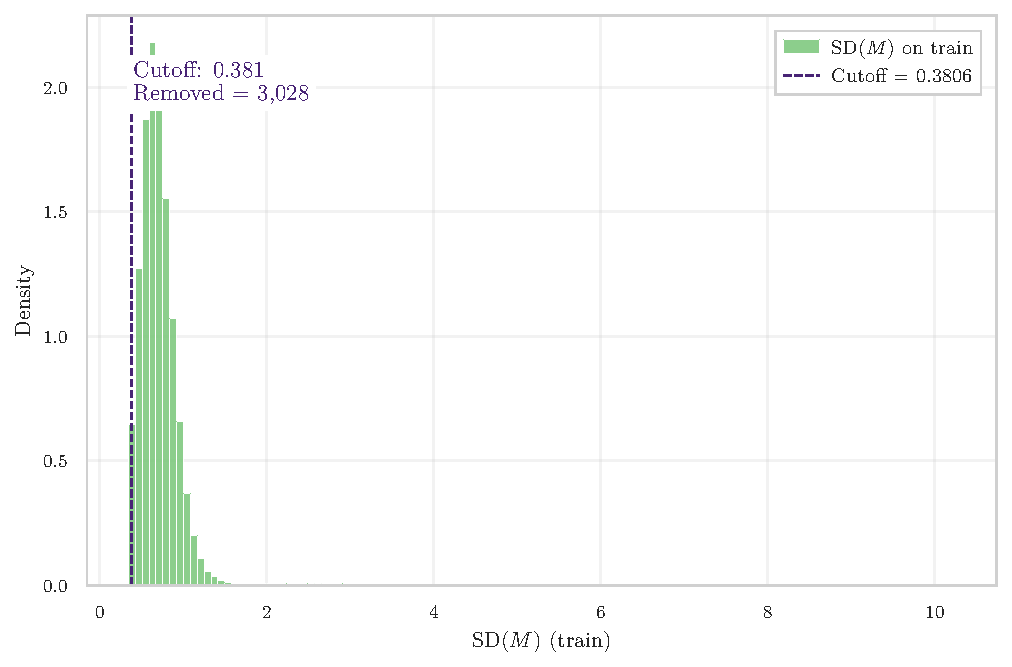
\includegraphics[width=\textwidth]{images/cap5/GSE69914_sdM_variance_filter.pdf}
    \caption{Distribution of $SD(M)$ on the training set. 
    The dashed line indicates the bottom 2\% quantile 
    used for residual variance trimming.}
    \label{fig:gse69914_sdM}
\end{subfigure}
\caption{Variability-based filtering in $\beta$-space and residual variance trimming in $M$-space in GSE69914.}
\label{fig:gse69914_variance_controls}
\end{figure}
% ============================================================


% ============================================================
\paragraph{Re-alignment to $M$-values and Residual Variance Regularisation}
% ============================================================

The retained CpGs were deterministically transformed to 
$M$-values, after which a residual low-variance trimming 
was applied in $M$-space. 
Figure~\ref{fig:gse69914_sdM} displays the distribution of 
empirical standard deviations $SD(M)$ on the training set.
The distribution is unimodal with limited heavy-tail behaviour. 
Removal of the bottom 2\% of CpGs by dispersion eliminated 
3{,}028 loci. 
Although quantitatively modest, this step improves covariance 
conditioning in the HDLSS regime.

% ============================================================
\paragraph{Biologically Weighted Stability Selection and Region-Level Consolidation}
% ============================================================

Repeated stratified resampling was used to estimate stability 
of signed mean differences. Figure~\ref{fig:gse69914_stability} 
shows the distribution of the directional stability score 
$S_{\mathrm{dir}}$.
The majority of CpGs exhibit high directional reproducibility, 
with substantial mass above 0.75. The threshold 
$\mathrm{stab}_j \geq 0.75$ excludes loci whose effect direction 
reverses across resampling splits, enforcing robustness 
consistent with the stability-selection principle of 
\cite{Meinshausen2010}.
After stability and adaptive effect-size filtering 
(60th percentile, corresponding to $|\Delta M| \approx 0.15$), 
the top 15{,}000 CpGs were retained by design, defining the 
candidate pool passed to correlation-based redundancy pruning.

% ============================================================
\begin{figure}[t]
\centering
\begin{subfigure}[t]{0.48\textwidth}
    \centering
    
\includegraphics[width=\textwidth]{images/cap5/GSE69914_stability_sign_distribution.pdf}
    \caption{Distribution of directional stability scores 
    $S_{\mathrm{dir}}$. The dashed line indicates the cutoff 
    $\mathrm{stab}_j \geq 0.75$.}
    \label{fig:gse69914_stability}
\end{subfigure}
\hfill
\begin{subfigure}[t]{0.48\textwidth}
    \centering
    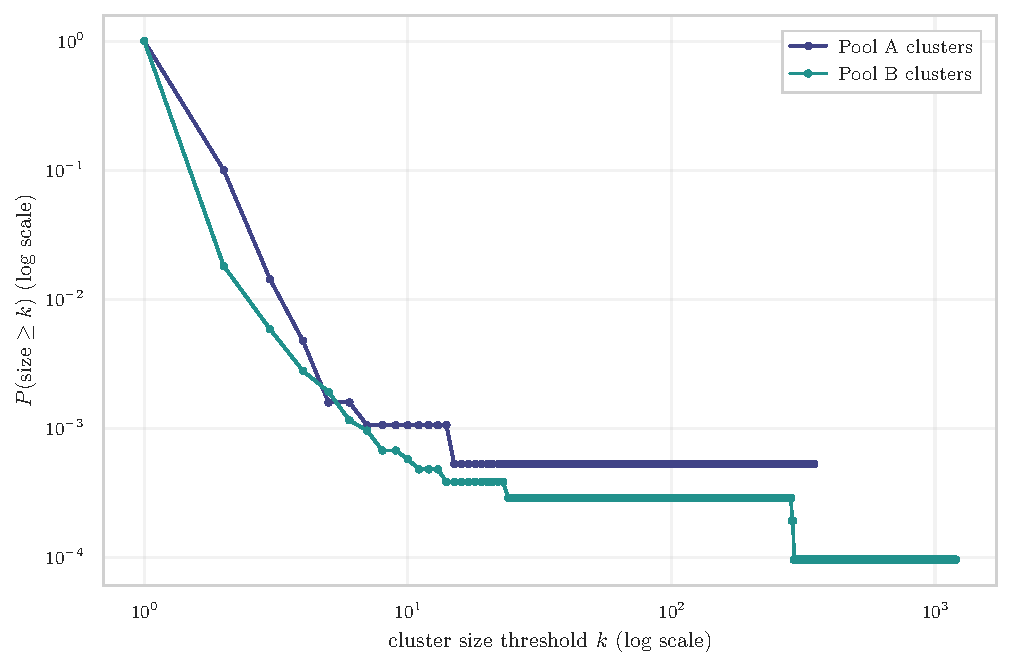
\includegraphics[width=\textwidth]{images/cap5/GSE69914_cluster_size_ccdf_loglog_r0_85.pdf}
    \caption{Cluster size survival curves for anchored (Pool A) 
    and non-anchored (Pool B) CpGs under $|r| \geq 0.85$.}
    \label{fig:gse69914_clusters}
\end{subfigure}
\caption{Stability enforcement and correlation-based redundancy structure in GSE69914.}
\label{fig:gse69914_stability_redundancy}
\end{figure}
% ============================================================

% ============================================================
\paragraph{Correlation-Based Redundancy Pruning and Graph-Theoretic Clustering}
% ============================================================

After stability and effect-size filtering, correlation-based 
graph clustering was applied separately to the anchored 
and non-anchored pools using a threshold of $|r| \ge 0.85$ 
computed on the training set. 
Figure~\ref{fig:gse69914_clusters} shows the cluster size 
survival curves, whose rapid decay indicates that most 
connected components are of size 1--3, reflecting limited 
local redundancy. Only a small number of large correlated blocks are 
observed, corresponding to densely co-methylated regions. 
Selecting a single representative CpG per component reduced 
the candidate space to 12{,}313 loci, defining the redundancy-pruned 
set passed to the diversification stage.

% ============================================================
\paragraph{Genomic Diversification via Constrained Greedy Selection}
% ============================================================

The constrained greedy diversification procedure selected 
$K=5000$ CpGs under chromosome, genomic context, and 
500kb spatial-window constraints. The strict 
constraint regime was sufficient to reach $K$ without requiring 
relaxation (maximum chromosome share 8\%, maximum 15 CpGs 
per 500kb window).
The final panel comprises 2{,}151 Island loci, 1{,}342 OpenSea loci, 
712 N\_Shore loci, 506 S\_Shore loci, and 150 N\_Shelf loci, 
indicating a diversified genomic-context composition rather than 
promoter-restricted enrichment. OpenSea loci were not excluded a priori, as distal regulatory 
regions may capture long-range epigenetic alterations relevant 
to early field effects.

% ============================================================
\begin{figure}[t]
\centering
\begin{subfigure}[t]{0.48\textwidth}
    \centering
    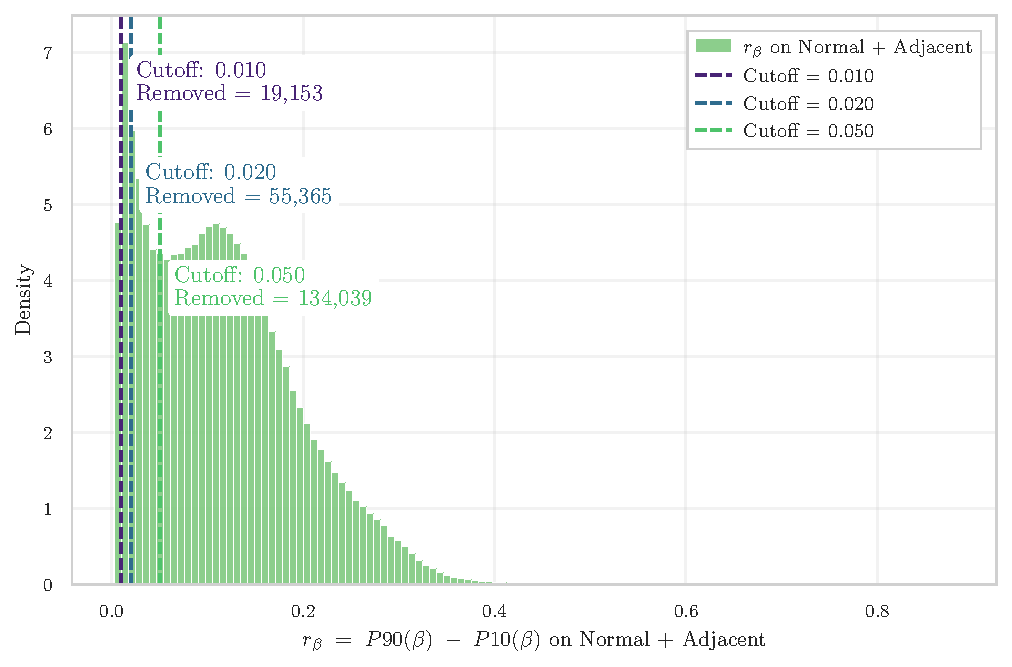
\includegraphics[width=\textwidth]{images/cap5/GSE225845_edgar_variability.pdf}
    \caption{$r_{\beta} = P90(\beta) - P10(\beta)$ 
    on the training set. Candidate thresholds 
    (0.01, 0.02, 0.05) are indicated.}
    \label{fig:gse225845_rbeta}
\end{subfigure}
\hfill
\begin{subfigure}[t]{0.48\textwidth}
    \centering
    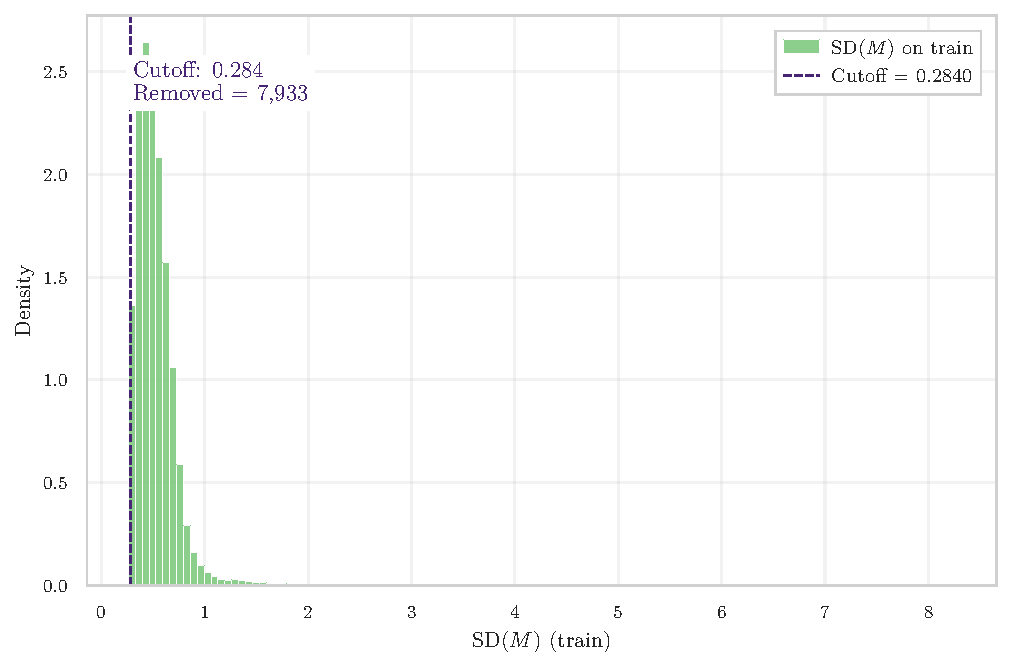
\includegraphics[width=\textwidth]{images/cap5/GSE225845_sdM_variance_filter.pdf}
    \caption{Distribution of $SD(M)$ on the training set. 
    The dashed line indicates the bottom 2\% quantile 
    used for residual variance trimming.}
    \label{fig:gse225845_sdM}
\end{subfigure}
\caption{Variability-based filtering in $\beta$-space and residual variance trimming in $M$-space in GSE225845.}
\label{fig:gse225845_variance_controls}
\end{figure}
% ============================================================


\subsection{Dataset GSE225845}
\label{subsec:fs_intra_gse225845}
The feature selection framework described in Section~\ref{sec:fs_framework} 
was applied to the preprocessed GSE225845 cohort, restricted to the 
Normal and Adjacent tissue classes, yielding a final panel of 
$K=5000$ CpGs after variability filtering, stability ranking, 
redundancy pruning, and diversification. The selected loci are 
available in the project repository at 
\href{https://github.com/elisabettaroviera/THESIS/blob/main/05%20-%20CpG%20list/Final%205000%20CpGs%20per%20Dataset/final_5000_gse225845.csv}
{\texttt{final\_5000\_gse225845.csv}}.

% ============================================================
\paragraph{Empirical Variability-Based Dimensionality Reduction}
% ============================================================

Variability was quantified via the inter-quantile range 
$r_{\beta,j} = P90(\beta) - P10(\beta)$ computed on the 
training set. Figure~\ref{fig:gse225845_rbeta} 
shows the empirical distribution of $r_{\beta}$ across CpGs. 
Applying the predefined threshold $\tau = 0.05$ removed 
134{,}039 low-variability loci, defining the reduced candidate 
space for downstream supervised ranking. Lower candidate 
thresholds (0.01, 0.02) are shown for reference but were not 
adopted. As observed in GSE69914, the variability-based reduction does 
not induce pathological genomic bias: invariant loci display 
moderate enrichment in promoter-proximal regions, while gene 
bodies and 3'UTR regions are relatively under-represented 
(see Appendix~\ref{app:empirical_variability_extension}).


% ============================================================
\paragraph{Re-alignment to $M$-values and Residual Variance Regularisation}
% ============================================================

The retained CpGs were deterministically transformed to 
$M$-values, after which a residual low-variance trimming 
was applied in $M$-space. 
Figure~\ref{fig:gse225845_sdM} displays the distribution of 
empirical standard deviations $SD(M)$ on the training set.
Removal of the bottom 2\% of CpGs by dispersion eliminated  
7{,}933 loci (cutoff $SD(M)=0.284$), defining the 
variance-regularised candidate space entering the 
stability-ranking stage.
% ============================================================
\paragraph{Biologically Weighted Stability Selection and Region-Level Consolidation}
% ============================================================

Repeated stratified resampling was used to estimate stability 
of signed mean differences. Figure~\ref{fig:gse225845_stability} 
shows the distribution of the directional stability score 
$S_{\mathrm{dir}}$.
The distribution is strongly right-skewed, with a substantial 
concentration of CpGs exhibiting $S_{\mathrm{dir}}$ close to 1, 
indicating highly consistent effect directions across resampling splits. 
The threshold $\mathrm{stab}_j \geq 0.75$ therefore removes only loci 
with unstable or sign-reversing effects, retaining the majority 
of directionally robust signals in this cohort.
After stability and adaptive effect-size filtering 
(60th percentile), the top 15{,}000 CpGs were retained by design, 
defining the candidate pool passed to correlation-based 
redundancy pruning.

% ============================================================
\begin{figure}[t]
\centering
\begin{subfigure}[t]{0.48\textwidth}
    \centering
    
\includegraphics[width=\textwidth]{images/cap5/GSE225845_stability_sign_distribution.pdf}
    \caption{Distribution of directional stability scores 
    $S_{\mathrm{dir}}$. The dashed line indicates the cutoff 
    $\mathrm{stab}_j \geq 0.75$.}
    \label{fig:gse225845_stability}
\end{subfigure}
\hfill
\begin{subfigure}[t]{0.48\textwidth}
    \centering
    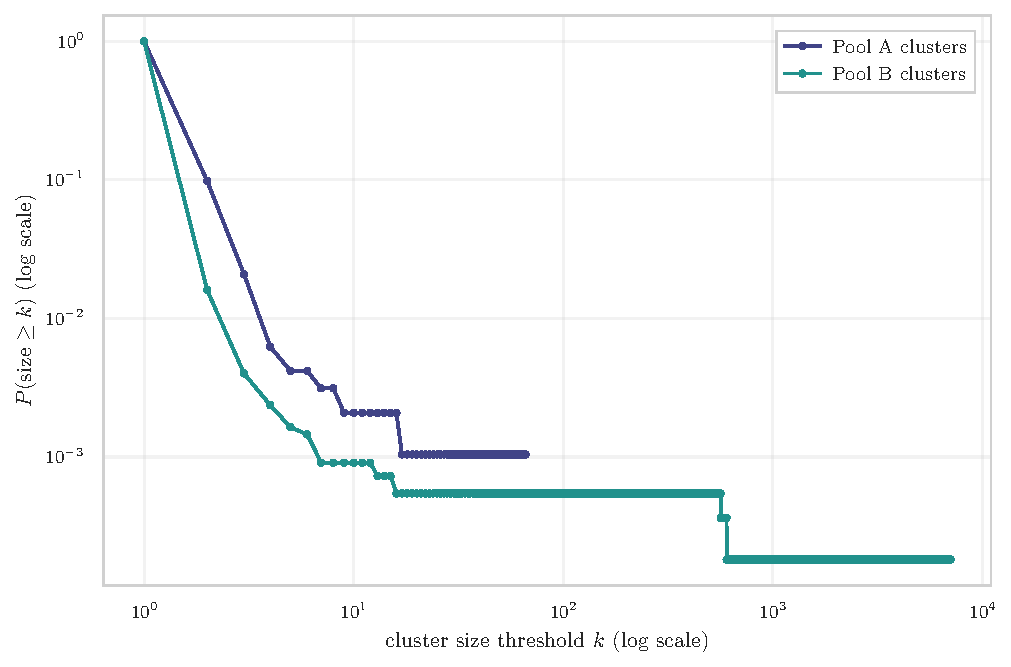
\includegraphics[width=\textwidth]{images/cap5/GSE225845_cluster_size_ccdf_loglog_r0_85.pdf}
    \caption{Cluster size survival curves for anchored (Pool A) 
    and non-anchored (Pool B) CpGs under $|r| \geq 0.85$.}
    \label{fig:gse225845_clusters}
\end{subfigure}
\caption{Stability and redundancy diagnostics in GSE225845.}
\label{fig:gse225845_stability_redundancy}
\end{figure}
% ============================================================


% ============================================================
\paragraph{Correlation-Based Redundancy Pruning and Graph-Theoretic Clustering}
% ============================================================

After stability and effect-size filtering, correlation-based 
graph clustering was applied separately to the anchored 
and non-anchored pools using a threshold of $|r| \ge 0.85$ 
computed on the training set. 
Figure~\ref{fig:gse225845_clusters} shows the cluster size 
survival curves.
The survival functions decay rapidly for small $k$, indicating 
that most connected components are of size 1--3. However, 
a pronounced heavy tail is observed, particularly in the 
non-anchored pool, with a limited number of large correlated 
blocks spanning tens to hundreds of CpGs.
This redundancy pruning step substantially reduced the 
candidate space from 15{,}000 to 6{,}453 loci, indicating 
a markedly higher correlation structure in GSE225845 
compared to GSE69914. The result suggests extended 
co-methylation domains consistent with the denser EPIC 
probe coverage.
Selecting a single representative CpG per connected component 
defines the redundancy-pruned set passed to the 
diversification stage.

% ============================================================
\paragraph{Genomic Diversification via Constrained Greedy Selection}
% ============================================================

The constrained greedy diversification procedure was applied 
to the 6{,}453 redundancy-pruned CpGs under chromosome, 
genomic-context, and 500kb spatial-window constraints. 
The strict constraint regime was sufficient to reach 
$K=5000$ without requiring relaxation 
(maximum chromosome share 8\%, maximum context share 65\%, 
maximum 15 CpGs per 500kb window).
The final panel comprises 2{,}115 Island loci, 1{,}746 OpenSea loci, 
534 N\_Shore loci, 436 S\_Shore loci, and 91 N\_Shelf loci, 
indicating a diversified genomic-context composition. 
The chromosome cap was actively binding in the strict stage, 
ensuring balanced genomic representation without overconcentration 
in high-density regions.
The resulting panel therefore satisfies all diversification 
constraints by construction.


\subsection{Dataset GSE287331}
\label{subsec:fs_intra_gse287331}


% ============================================================
\begin{figure}[t]
\centering
\begin{subfigure}[t]{0.48\textwidth}
    \centering
    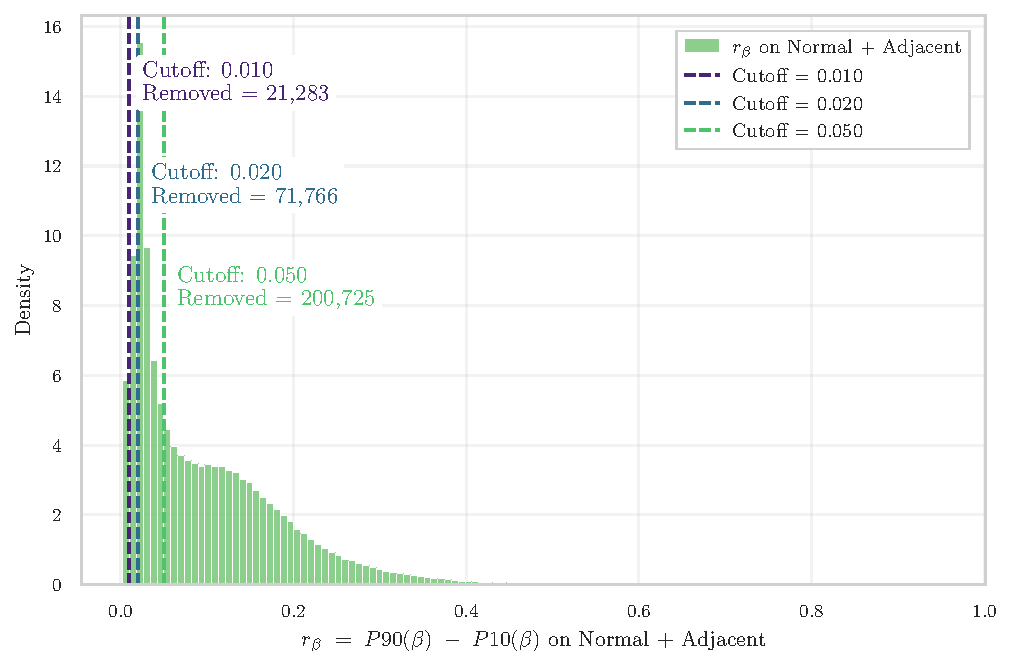
\includegraphics[width=\textwidth]{images/cap5/GSE287331_edgar_variability.pdf}
    \caption{$r_{\beta} = P90(\beta) - P10(\beta)$ 
    on the training set. Candidate thresholds 
    (0.01, 0.02, 0.05) are indicated.}
    \label{fig:gse287331_rbeta}
\end{subfigure}
\hfill
\begin{subfigure}[t]{0.48\textwidth}
    \centering
    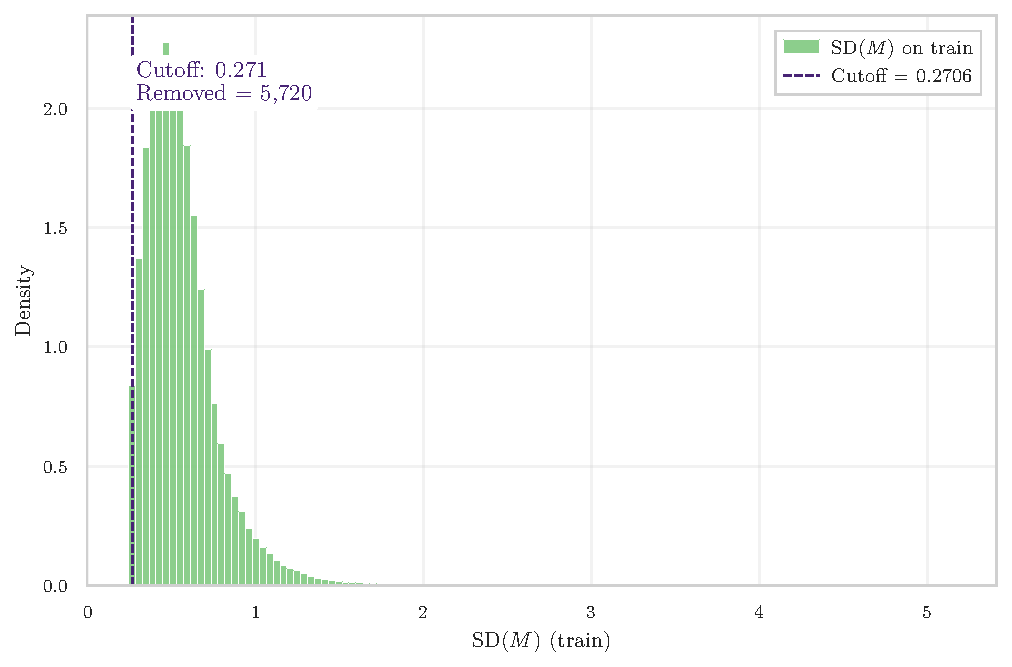
\includegraphics[width=\textwidth]{images/cap5/GSE287331_sdM_variance_filter.pdf}
    \caption{Distribution of $SD(M)$ on the training set. 
    The dashed line indicates the bottom 2\% quantile 
    used for residual variance trimming.}
    \label{fig:gse287331_sdM}
\end{subfigure}
\caption{Variability-based filtering in $\beta$-space and residual variance trimming in $M$-space in GSE287331.}
\label{fig:gse287331_variance_controls}
\end{figure}
% ============================================================


The feature selection framework described in Section~\ref{sec:fs_framework} 
was applied to the preprocessed GSE287331 cohort, restricted to the 
Normal and Adjacent tissue classes, yielding a final panel of 
$K=5000$ CpGs after variability filtering, stability ranking, 
redundancy pruning, and diversification. The selected loci are 
available in the project repository at 
\href{https://github.com/elisabettaroviera/THESIS/blob/main/05%20-%20CpG%20list/Final%205000%20CpGs%20per%20Dataset/final_5000_gse287331.csv}
{\texttt{final\_5000\_gse287331.csv}}.

% ============================================================
\paragraph{Empirical Variability-Based Dimensionality Reduction}
% ============================================================

Variability was quantified via the inter-quantile range 
$r_{\beta,j} = P90(\beta) - P10(\beta)$ computed on the 
training set. Figure~\ref{fig:gse287331_rbeta} 
shows the empirical distribution of $r_{\beta}$ across CpGs, 
which is heavily concentrated near zero, indicating a large 
fraction of weakly variable loci.
Applying the predefined threshold $\tau = 0.05$ removed 
200{,}725 low-variability CpGs, substantially reducing the 
dimensionality of the feature space prior to supervised ranking. 
Lower candidate thresholds are shown for reference 
but were not adopted, as they would retain a markedly larger 
proportion of near-constant probes. Consistent with the other cohorts, invariant CpGs exhibit 
moderate enrichment in promoter-proximal regions (notably TSS200 
and first exon), while distal or non-promoter regions are 
relatively under-represented (see Appendix~\ref{app:empirical_variability_extension}). 
The magnitude of enrichment is less pronounced than in 
GSE69914 and GSE225845, suggesting that the variability structure 
of this dataset is more diffusely distributed across genomic 
contexts.


% ============================================================
\paragraph{Re-alignment to $M$-values and Residual Variance Regularisation}
% ============================================================

The retained CpGs were deterministically transformed to 
$M$-values, after which a residual low-variance trimming 
was applied in $M$-space. 
Figure~\ref{fig:gse287331_sdM} displays the distribution of 
empirical standard deviations $SD(M)$ on the training set, 
which is unimodal with moderate right-tail behaviour.
Removal of the bottom 2\% of CpGs by dispersion 
(cutoff $SD(M)=0.271$) eliminated 5{,}720 loci, 
defining the variance-regularised candidate space entering 
the stability-ranking stage.

% ============================================================
\begin{figure}[t]
\centering
\begin{subfigure}[t]{0.48\textwidth}
    \centering
    
\includegraphics[width=\textwidth]{images/cap5/GSE287331_stability_sign_distribution.pdf}
    \caption{Distribution of directional stability scores 
    $S_{\mathrm{dir}}$. The dashed line indicates the cutoff 
    $\mathrm{stab}_j \geq 0.75$.}
    \label{fig:gse287331_stability}
\end{subfigure}
\hfill
\begin{subfigure}[t]{0.48\textwidth}
    \centering
    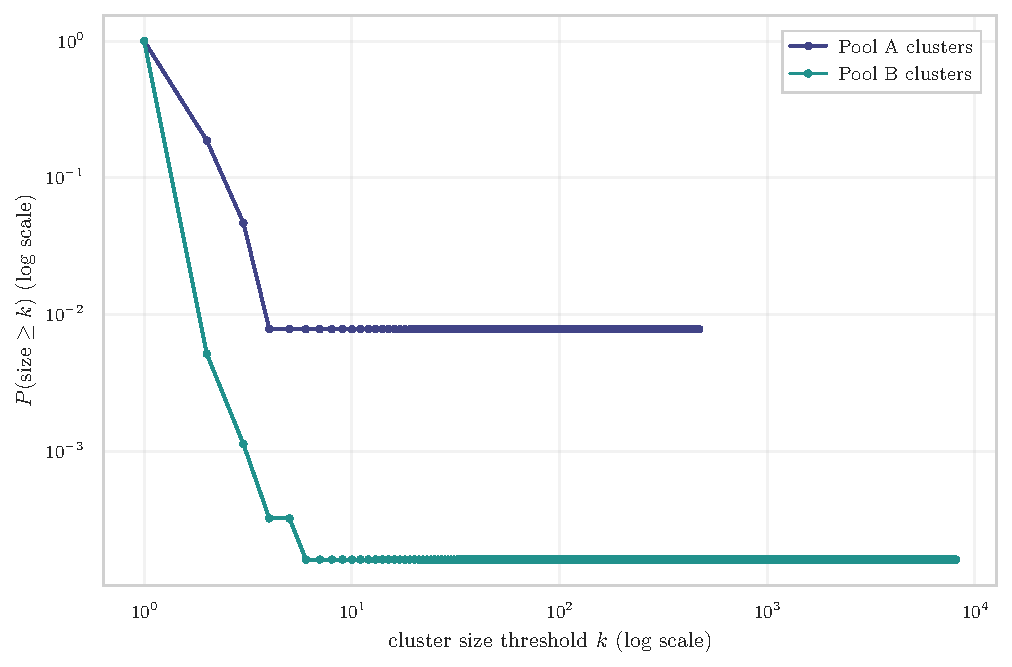
\includegraphics[width=\textwidth]{images/cap5/GSE287331_cluster_size_ccdf_loglog_r0_85.pdf}
    \caption{Cluster size survival curves for anchored (Pool A) 
    and non-anchored (Pool B) CpGs under $|r| \geq 0.85$.}
    \label{fig:gse287331_clusters}
\end{subfigure}
\caption{Stability and redundancy diagnostics in GSE287331.}
\label{fig:gse287331_stability_redundancy}
\end{figure}
% ============================================================


% ============================================================
\paragraph{Biologically Weighted Stability Selection and Region-Level Consolidation}
% ============================================================

Repeated stratified resampling was used to estimate stability 
of signed mean differences. Figure~\ref{fig:gse287331_stability} 
shows the distribution of the directional stability score 
$S_{\mathrm{dir}}$, which is sharply concentrated near 1. 
A pronounced peak at high stability values indicates that 
the vast majority of CpGs exhibit highly consistent effect 
directions across resampling splits.
The threshold $\mathrm{stab}_j \geq 0.75$ therefore removes 
only a small subset of unstable loci, enforcing directional 
robustness in line with the stability-selection principle 
of~\cite{Meinshausen2010} while retaining most candidate signals.
After stability and adaptive effect-size filtering 
(60th percentile), the top 15{,}000 CpGs were retained by design, 
defining the candidate pool passed to correlation-based 
redundancy pruning.


% ============================================================
\paragraph{Correlation-Based Redundancy Pruning and Graph-Theoretic Clustering}
% ============================================================

After stability and effect-size filtering, correlation-based 
graph clustering was applied separately to the anchored 
and non-anchored pools using a threshold of $|r| \ge 0.85$ 
computed on the training set. 
Figure~\ref{fig:gse287331_clusters} shows the cluster size 
survival curves.
The survival functions exhibit a rapid decay, indicating that 
most connected components are of size 1--3 and that large 
correlated blocks are rare. Compared to GSE225845, the absence 
of a pronounced heavy tail suggests a more locally structured 
correlation pattern without extended co-methylation domains.
Selecting a single representative CpG per connected component 
reduced the candidate space to 6{,}300 loci, defining the 
redundancy-pruned set passed to the diversification stage.

% ============================================================
\paragraph{Genomic Diversification via Constrained Greedy Selection}
% ============================================================

The constrained greedy diversification procedure was applied 
to the 6{,}300 redundancy-pruned CpGs under chromosome, 
genomic-context, and 500kb spatial-window constraints. 
The strict constraint regime was sufficient to reach 
$K=5000$ without requiring relaxation.
The final panel comprises 1{,}992 OpenSea loci, 1{,}692 Island loci, 
556 N\_Shore loci, 507 S\_Shore loci, and 135 S\_Shelf loci, 
indicating a diversified genomic-context composition with a 
substantial contribution from distal regions.

%----------------------------------------------------------------------
\begin{figure}[t]
    \centering
    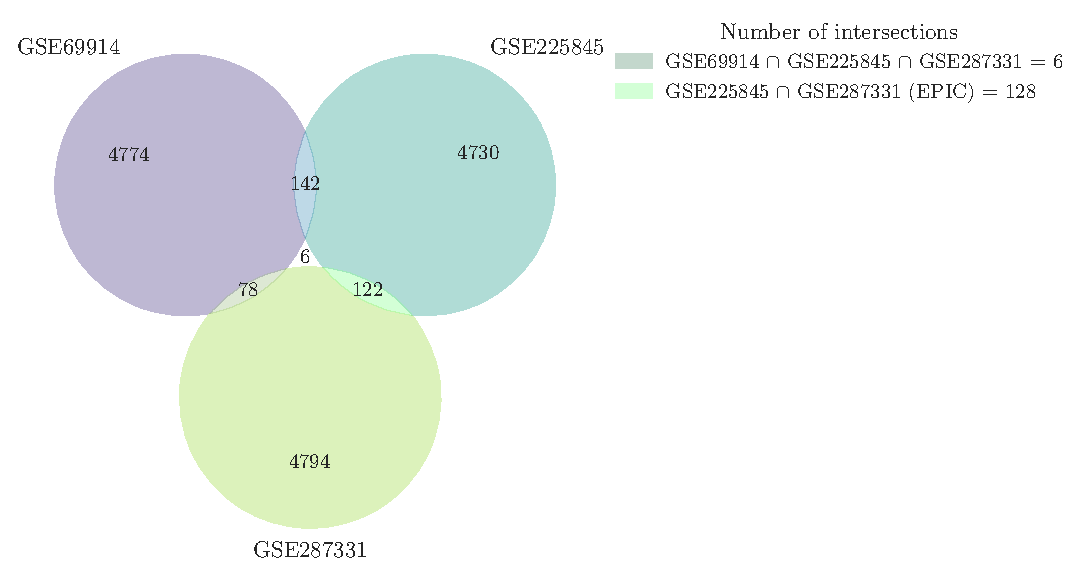
\includegraphics[width=0.75\textwidth]
    {images/cap5/FINAL5000_CpG_overlap_venn3.pdf}
    
    \caption{Three-way overlap of the final 5{,}000 CpG signatures
    independently selected in GSE69914, GSE225845 and GSE287331.
    }
    
    \label{fig:interfs_venn}
\end{figure}
%----------------------------------------------------------------------


%======================================================================
\section{Inter-Dataset Stability of the Final 5{,}000 CpG Signatures}
\label{sec:inter_dataset_fs}
%======================================================================

The feature selection framework described in Section~\ref{sec:fs_intra_dataset}
was applied independently to each cohort, yielding three dataset-specific
panels of $K = 5{,}000$ CpG loci optimised for within-dataset discrimination
along the Normal--Adjacent axis.
The present section quantifies the degree to which these panels converge
on a shared epigenetic drift signal, thereby assessing the cross-cohort
replicability of the feature selection outcome.
Consistency is evaluated at three complementary levels:
(i) identity-level overlap of selected loci (set-level replicability),
(ii) concordance of estimated effect sizes across cohort intersections
(effect-level agreement), and
(iii) transferability of the drift structure as a discriminative ranking
in held-out datasets.
This multi-resolution framework mirrors the analytical strategy adopted
for the pre-selection inter-dataset analysis of Section~\ref{sec:fs_intra_dataset},
now applied to the output of the full selection pipeline rather than to
the global methylome.


%----------------------------------------------------------------------
\subsection{Set-Level Replicability}
\label{sec:inter_fs_overlap}
%----------------------------------------------------------------------

\begin{table}[t]
\centering
\scriptsize
\caption{Permutation-based enrichment of pairwise overlaps among the three final $5{,}000$-CpG panels.}
\label{tab:interfs_overlap}
\begin{tabular}{l c c c c}
\toprule
Pair & Shared CpGs & Expected Overlap & Enrichment Ratio & $p$-value \\
\midrule
GSE69914--GSE225845 & 148 & 69.0 & $2.14$ & $< 10^{-4}$ \\
GSE69914--GSE287331 &  84 & 68.3 & $1.23$ & $0.024$     \\
GSE225845--GSE287331 & 128 & 37.9 & $3.38$ & $< 10^{-4}$ \\
\bottomrule
\end{tabular}
\end{table}
Pairwise intersections between the three final $5{,}000$-CpG panels were
computed and are visualised in Figure~\ref{fig:interfs_venn}.
The identity-level overlap is summarised by the Jaccard similarity
coefficient, which for two selection sets $A$ and $B$ is defined as
\begin{equation}
    J(A,B) = \frac{|A \cap B|}{|A \cup B|},
    \label{eq:jaccard}
\end{equation}
where $|A \cap B|$ denotes the cardinality of the shared loci and
$|A \cup B|$ the size of their union.
This scale-invariant measure normalises the raw intersection count
against the total selection universe, rendering it comparable across
cohort pairs with different platform intersections.
The observed values,
\(
J(\text{GSE69914},\text{GSE225845}) = 0.0150,\)
\(J(\text{GSE69914},\text{GSE287331}) = 0.0085,\)
\(J(\text{GSE225845},\text{GSE287331}) = 0.0130,
\)
indicate that fewer than $1.5\%$ of selected CpGs are shared between
any two cohort-specific panels, confirming that identity-level
replicability is limited across all pairs.
This pattern is consistent with the weak locus-level reproducibility
observed in the pre-selection inter-dataset analysis
(Section~\ref{sec:inter_dataset}).
Given the high-dimensional setting, cohort-specific noise structure,
and heterogeneous sampling conditions, only partial overlap
between independently derived panels is expected.

\paragraph{Permutation-based assessment of overlap significance}
A naive interpretation of the raw intersection size would be
misleading without accounting for the baseline expected overlap
under random selection.
The appropriate null model must reflect the actual constraints of
the selection procedure: each panel draws exactly $K = 5{,}000$
CpGs from its own post-preprocessing feature space, and the two
panels can only share loci that are present in \emph{both} datasets
after platform-specific filtering.
The effective sampling universe for each pair is therefore the
post-preprocessing pairwise intersection $\mathcal{U}_{AB} =
\mathcal{C}_A \cap \mathcal{C}_B$, where $\mathcal{C}_A$ and
$\mathcal{C}_B$ denote the full sets of CpGs retained after
preprocessing in datasets $A$ and $B$, respectively.
Under this null, $10{,}000$ independent replications were generated
by drawing two sets of $K = 5{,}000$ CpGs uniformly at random from
$\mathcal{U}_{AB}$, without replacement, and recording their
intersection size.
The empirical $p$-value is defined as the proportion of replications
in which the random overlap equals or exceeds the observed value.
This construction is conservative relative to null models based on
the full genome or on the union of platform probes, since the
restricted universe $\mathcal{U}_{AB}$ raises the baseline expected
overlap; significance under this test therefore provides a more
stringent criterion for enrichment.
Results are reported in Table~\ref{tab:interfs_overlap}.
All three pairwise overlaps exceed the permutation null at nominal
significance.
The most pronounced enrichment is observed for the EPIC--EPIC pair
(GSE225845--GSE287331; enrichment $\times 3.4$), reflecting the
larger shared platform intersection available to that pair.
The HM$450$--EPIC pairs yield smaller but still significant
enrichments, indicating that the selection procedure recovers a
non-random shared subset even across platform boundaries.

Importantly, statistical significance here quantifies enrichment
relative to the large-cardinality random baseline, and should not
be conflated with biological equivalence of the selected panels.
The restricted sampling universe $\mathcal{U}_{AB}$ is itself of
order $\mathcal{O}(10^5)$, so even modest absolute overlaps can
achieve nominal significance when drawn from such a large pool.
Jaccard indices below $0.02$ demonstrate that fewer than one in
fifty selected CpGs is reproducibly identified across independent
cohorts, and that identity-level concordance is insufficient to
constitute a shared genomic signature.
Cross-cohort replicability must therefore be evaluated at the level
of effect structure rather than probe identity, as formalised in
the following subsections.

%----------------------------------------------------------------------
\begin{figure}[t]
    \centering
    
    \begin{subfigure}{0.48\textwidth}
        \centering
        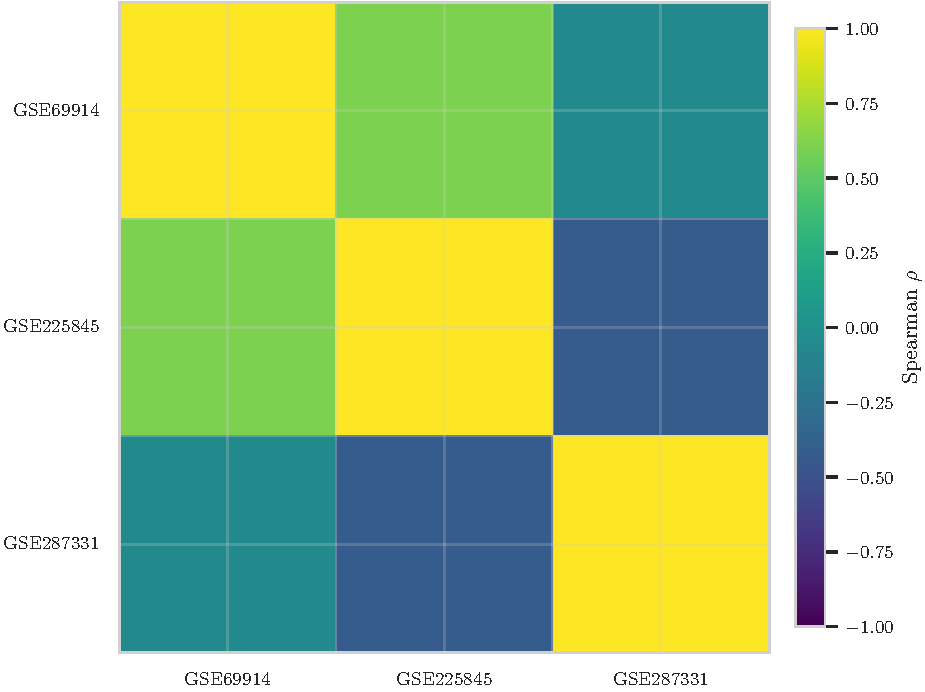
\includegraphics[width=\textwidth]
        {images/cap5/InterFS_concordance_matrix_spearman_rho.pdf}
        \caption{Spearman correlation $\rho$ of $\Delta\beta$}
        \label{fig:interfs_rho}
    \end{subfigure}
    \hfill
    \begin{subfigure}{0.48\textwidth}
        \centering
        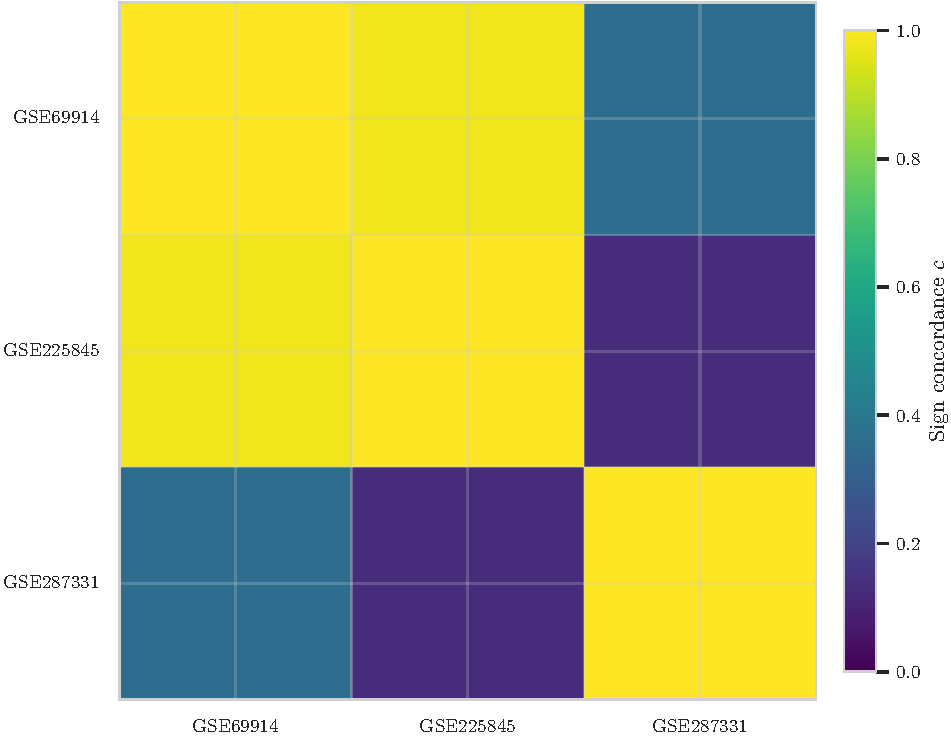
\includegraphics[width=\textwidth]
        {images/cap5/InterFS_concordance_matrix_sign_concordance.pdf}
        \caption{Sign concordance $c$}
        \label{fig:interfs_sign}
    \end{subfigure}
    
    \caption{Inter-dataset effect concordance of the final 5{,}000 CpG signatures. 
}
    
    \label{fig:interfs_concordance}
\end{figure}
%----------------------------------------------------------------------

%----------------------------------------------------------------------
\subsection{Effect-Direction Concordance}
\label{sec:inter_fs_effect}
%----------------------------------------------------------------------

The absence of strong identity-level overlap does not preclude the
existence of a shared differential methylation structure: independently
selected panels may still converge on the same underlying drift axis if
the corresponding effect sizes are concordant across cohorts.
To evaluate this possibility, signed mean methylation differences
$\Delta\beta_j = \bar{\beta}^{\text{Adj}}_j - \bar{\beta}^{\text{Norm}}_j$
were computed for each CpG $j$ in the pairwise intersection of the
respective $5{,}000$-CpG panels.
Concordance was assessed through two complementary measures:
the Spearman rank correlation $\rho$ of signed effect sizes, which
captures both magnitude and direction, and the directional concordance
rate
\begin{equation}
  c = \widehat{\mathbb{P}}\!\left(\operatorname{sign}(\Delta\beta^{(A)}_j)
  = \operatorname{sign}(\Delta\beta^{(B)}_j)\right),
  \label{eq:sign_concordance}
\end{equation}
estimated with Wilson confidence intervals, which isolates the
directional component independently of magnitude.
The distinction between $\rho$ and $c$ is methodologically important:
a low signed correlation combined with high directional concordance
indicates attenuated but direction-preserving effects, whereas negative
$\rho$ accompanied by $c \ll 0.5$ is diagnostic of systematic polarity
inversion rather than mere amplitude attenuation.
Both quantities are visualised jointly in
Figure~\ref{fig:interfs_concordance}.

\paragraph{GSE69914--GSE225845: shared drift axis}
The HM$450$--EPIC pair exhibits strong positive rank correlation
($\rho = 0.605$) and near-complete directional alignment
($c = 0.980$, Wilson 95\% CI excluded from $0.5$ by a wide margin).
Together, these values indicate that the two datasets not only
agree on the direction of each locus-specific shift but also
preserve the relative ordering of effect magnitudes.
This constitutes the clearest evidence of a shared epigenetic
drift axis across independent cohorts, despite the known
platform heterogeneity between the HM$450$ and EPIC arrays.

\paragraph{GSE287331: systematic polarity inversion}
Pairs involving GSE287331 display a qualitatively distinct pattern.
The Spearman correlations are weakly negative
($\rho = -0.042$ with GSE69914; $\rho = -0.420$ with GSE225845),
and directional concordance falls substantially below $0.5$
($c = 0.357$ and $c = 0.125$, respectively).
The value $c = 0.125$ in particular implies that only one in
eight selected CpGs shares the same Adjacent--Normal polarity
between GSE225845 and GSE287331, a pattern incompatible with
stochastic disagreement and indicative of a systematic reversal
of the dominant drift direction.
Crucially, this inversion is not attributable to the absence of a
discriminative signal in GSE287331: the intra-dataset analyses of
Section~\ref{sec:fs_intra_dataset} demonstrated that this cohort
yields the strongest and most geometrically coherent Normal--Adjacent
separation of the three (silhouette $= 0.3442$; outlier A/N ratio
$= 13.3$).
Rather, the inversion reflects a structural asymmetry in the
orientation of the drift manifold, likely arising from a combination
of platform-specific probe-type composition, the distinct
tumour-proximity sampling design of GSE287331 (TPxA axis), and
residual confounding by cohort-specific batch structure.

%----------------------------------------------------------------------
\subsection{Magnitude-Stratified Concordance}
\label{sec:inter_fs_magnitude}
%----------------------------------------------------------------------

The signed and directional analyses of Section~\ref{sec:inter_fs_effect}
characterise the global behaviour of effect sizes across the pairwise
intersection of selected panels.
A complementary question is whether concordance is uniform across the
effect magnitude spectrum or, rather, whether it is concentrated in loci
exhibiting the strongest drift signals — a distinction with direct
implications for the biological interpretability of cross-cohort
consistency.
To address this, CpGs in the pairwise intersection were stratified by
decile of absolute effect magnitude $|\Delta\beta|$, computed
independently in each dataset.
For each decile bin, the fraction of loci whose effect direction agreed
across cohorts was computed, yielding a magnitude-stratified directional
concordance profile.

For the GSE69914--GSE225845 pair, directional concordance is high and
stable across all deciles, with no systematic attenuation in lower-magnitude
strata.
Crucially, the top decile — comprising CpGs with the largest
$|\Delta\beta|$ in both datasets — exhibits the highest concordance,
indicating that the strongest signals are preferentially shared.
This behaviour supports the interpretation that the cross-cohort
agreement between these two datasets is not an artefact of
magnitude-insensitive directional alignment, but reflects a genuinely
shared structure concentrated at loci with the most pronounced
Adjacent--Normal differential methylation.

Pairs involving GSE287331 display a markedly different pattern.
Directional concordance remains depressed across all decile strata,
with no recovery in the high-magnitude bins.
This rules out the scenario in which directionality disagreement
would be confined to low-amplitude, noisy loci — as would be
expected under pure stochastic disagreement — and instead confirms
that the inversion of effect orientation is structural and affects
loci of all effect magnitudes, including those most strongly
discriminative within GSE287331.
Taken together with the negative signed correlations reported in
Section~\ref{sec:inter_fs_effect}, this evidence positions the
GSE287331 discordance firmly in the \emph{directional inversion}
regime rather than the \emph{structural heterogeneity} regime
of Section~\ref{sec:fs_conclusion}: the selected loci
are not uninformative, but their dominant drift axis is systematically
rotated relative to that of the other two cohorts.

%----------------------------------------------------------------------
\subsection{Cross-Dataset Transferability}
\label{sec:inter_fs_transfer}
%----------------------------------------------------------------------

Set-level overlap and effect-level concordance characterise the
structure of the selected panels on their own terms.
A more stringent criterion for cross-cohort replicability is
\emph{functional transferability}: whether the differential methylation
signal inferred in one cohort retains discriminative power when applied
to an independent dataset, without any retraining or adaptation.
Formally, for each ordered pair of datasets $(A, B)$, a linear scoring
function $f^{(A)}: \mathbb{R}^{|S_{AB}|} \to \mathbb{R}$ was defined on
the intersection $S_{AB}$ of the respective $5{,}000$-CpG panels, using
the cohort-$A$ effect sizes $\Delta\beta^{(A)}$ as fixed coefficients:
\begin{equation}
  f^{(A)}(\mathbf{x}^{(B)}_i) = \sum_{j \in S_{AB}}
  \Delta\beta^{(A)}_j \cdot x^{(B)}_{ij},
  \label{eq:transfer_score}
\end{equation}
where $\mathbf{x}^{(B)}_i$ denotes the methylation profile of sample $i$
in dataset $B$.
This zero-shot transfer procedure isolates the intrinsic portability of
the drift structure itself, independent of classifier fitting.
Discriminative performance was evaluated via the area under the
ROC curve (AUC), with values near $0.5$ indicating absence of transfer,
values substantially above $0.5$ indicating directionally consistent
transfer, and values substantially below $0.5$ indicating systematic
inversion — i.e.\ the scoring function trained on cohort $A$ assigns
\emph{higher} scores to Normal than to Adjacent samples in cohort $B$.

\paragraph{GSE69914--GSE225845}
Bidirectional transfer between the HM$450$ and EPIC cohorts was 
evaluated by training a univariate $\Delta\beta$ ranking rule in one 
dataset and applying it directly to the other. 
Specifically, given an effect-size vector $\Delta\beta$ estimated 
in the source cohort, each sample $x$ in the target cohort was 
assigned the discriminative score:
\begin{equation}
s(x) = \sum_{j \in \mathcal{S}} \Delta\beta_j \, x_j ,
\end{equation}
where $\mathcal{S}$ denotes the selected CpG panel and $x_j$ the 
methylation level of locus $j$. 
No re-estimation or adaptation to the target distribution was performed.
Discriminative performance was quantified via the area under the 
receiver operating characteristic curve (AUC), defined as
\begin{equation}
\mathrm{AUC}
=
\int_0^1 \mathrm{TPR}(t)\, d\mathrm{FPR}(t),
\end{equation}
where $\mathrm{TPR}$ and $\mathrm{FPR}$ denote the true- and false-positive 
rates across classification thresholds. 
For the binary Normal–Adjacent problem, this quantity is 
equivalently expressed as
\begin{equation}
\mathrm{AUC}
=
\mathbb{P}\!\left(
s(X_{A}) > s(X_{N})
\right),
\end{equation}
that is, the probability that a randomly selected Adjacent sample 
receives a higher score than a randomly selected Normal sample. 
The AUC takes values in $[0,1]$, where $0.5$ corresponds to 
chance-level discrimination, values above $0.5$ indicate 
discriminative ability in the correct direction, and $1$ 
corresponds to perfect separation. Values below $0.5$ 
reflect systematic inversion of the ranking rule.

The resulting AUC was $0.776$ when training on GSE69914 and 
testing on GSE225845, and $0.794$ in the reverse direction. 
Both values are substantially above chance, indicating that the 
shared drift axis identified through concordance analysis 
translates into genuine discriminative transferability. 
These results provide the strongest cross-cohort evidence in 
the present study that the GSE69914--GSE225845 pair captures 
a reproducible and functionally portable epigenetic drift structure.

\paragraph{Transfers involving GSE287331}
All four directed transfer pairs involving GSE287331 yield AUC values
in the range $[0.017,\, 0.226]$, substantially and consistently below
chance level.
Sub-random AUC is not a failure of discriminability per se, but rather
a signature of systematic directional inversion: the scoring function
derived from one cohort actively misranks samples in the other,
assigning higher drift scores to the tissue class with lower methylation
deviation.
This outcome is the functional counterpart of the near-zero or negative
sign concordance ($c = 0.125$--$0.357$) and negative Spearman correlations
($\rho = -0.042$ to $-0.420$) reported in Section~\ref{sec:inter_fs_effect},
and provides definitive evidence that the polarity inversion observed at
the descriptive level has concrete consequences for predictive transfer.

\paragraph{Interpretation}
The transferability results complete the multi-level concordance portrait
of the three selected panels.
The GSE69914--GSE225845 pair satisfies all criteria for the
\emph{shared drift structure} regime: significant set enrichment,
high directional concordance, magnitude-stratified agreement concentrated
at strong-effect loci, and bidirectional AUC well above chance.
Pairs involving GSE287331 are consistent with the
\emph{directional inversion} regime: non-trivial set enrichment,
systematically inverted effect polarity across all magnitude strata,
and sub-random transfer performance.
These asymmetries have direct methodological consequences for the
downstream modelling strategy developed in Chapter~\ref{chap:model_training_evaluation}:
naive cross-cohort transfer from or to GSE287331 is not only
non-informative but actively misleading, motivating the need for
orientation-aware or cohort-adaptive learning approaches.

%----------------------------------------------------------------------
\begin{table}[t]
\centering
\scriptsize
\caption{Number of CpGs retained at each step of the feature selection pipeline (training set).}
\label{tab:fs_reduction_steps_all}
\begin{tabular}{l c c c}
\toprule
Pipeline step 
& CpGs in GSE69914 
& CpGs in GSE225845 
& CpGs in GSE287331 \\
\midrule
Post-preprocessing space           & 251{,}483 & 530{,}683 & 486{,}725 \\
After Edgar variability filter     & 151{,}380 & 396{,}644 & 286{,}000 \\
After $M$-value SD trimming        & 148{,}352 & 388{,}711 & 280{,}280 \\
After stability + effect-size filter
                                   & 15{,}000  & 15{,}000  & 15{,}000  \\
After correlation pruning          & 12{,}313  & 6{,}453   & 6{,}300  \\
After constrained diversification  & 5{,}000   & 5{,}000   & 5{,}000   \\
\bottomrule
\end{tabular}
\end{table}
%----------------------------------------------------------------------


% ============================================================
\section{Feature Selection Outcomes and Modelling Implications}
\label{sec:fs_conclusion}
% ============================================================

The feature selection framework developed in this chapter addresses
the core challenge posed by genome-wide DNA methylation data in the
HDLSS regime: identifying a compact, stable, and biologically coherent
CpG panel capable of characterising the Normal--Adjacent transition
across independent cohorts.
The pipeline applies strictly train-only dimensionality reduction
stages, each targeting a distinct source of noise or redundancy.
Table~\ref{tab:fs_reduction_steps_all} summarises the progressive
reduction from post-preprocessing spaces of $251{,}483$--$530{,}683$
CpGs to final panels of $K = 5{,}000$ loci. The resulting panels
exhibit directional stability scores concentrated near unity,
indicating reproducible Adjacent--Normal polarity across resampling
splits; correlation pruning eliminates co-methylated blocks; and
genomic diversification enforces broad chromosomal and
regulatory-context coverage.
The inter-dataset evaluation of Section~\ref{sec:inter_dataset_fs}
reveals partial and asymmetric cross-cohort replicability.
GSE69914 and GSE225845 satisfy the \emph{shared drift structure}
regime: their panels are mutually enriched beyond chance, exhibit
near-complete directional concordance ($c = 0.980$), and support
bidirectional zero-shot transfer (AUC $= 0.776$ and $0.794$).
GSE287331, by contrast, occupies the \emph{directional inversion}
regime: its panel captures a robust but systematically inverted
drift axis, yielding sub-random transfer performance
(AUC $\in [0.017,\, 0.226]$) against both partner cohorts.
This asymmetry implies that linear $\Delta\beta$ signatures,
however stable within a cohort, do not constitute a universally
portable representation of the Normal--Adjacent transition.

These structural properties and cross-cohort limitations jointly
define the downstream modelling strategy. Within each cohort, the
selected panels provide a stability-filtered input for supervised
Normal--Adjacent classification, evaluated in
Chapter~\ref{chap:model_training_evaluation}. Where drift
orientation is preserved — as between GSE69914 and GSE225845 —
cross-dataset transfer is a principled objective; where systematic
inversion is present, orientation-aware strategies are required.
Chapter~\ref{chap:multi_cohort_integration} addresses this through
multi-cohort pooling and biological synthesis, investigating whether
signal consolidation across heterogeneous cohorts supports a more
robust characterisation of the Normal--Adjacent transition despite
divergent drift orientations.